\documentclass[wes, manuscript]{copernicus}
\usepackage{lineno}
\modulolinenumbers[1]
% --------------------------------------------------------------------------------}
% --- USER COMMANDS 
% --------------------------------------------------------------------------------{
\usepackage{graphicx}
\usepackage[super]{nth}
%\usepackage[colorlinks,bookmarksopen,bookmarksnumbered,citecolor=red,urlcolor=red]{hyperref}
\usepackage{amsmath}
\usepackage{amssymb}
\usepackage{amsthm}
\usepackage{mathtools}
\usepackage{import}
%\usepackage{xcolor} 
\hypersetup{
    colorlinks = false,
    linkcolor =[rgb]{0.2,0.2,0.2},
    linkbordercolor =[rgb]{0.7,0.7,0.7}
}
\providecommand{\tightlist}{\setlength{\itemsep}{0pt}\setlength{\parskip}{0pt}}
% --- Maths
\newcommand{\eqdef}{\stackrel{\mathsmaller{\mathsmaller{\mathsmaller{\triangle}}}}{=}} 
\renewcommand{\d}{\mathrm{d}}
\renewcommand{\v}[1]{\boldsymbol{#1}}
\newcommand{\m}[1]{\boldsymbol{#1}}
\providecommand{\norm}[1]{\lVert#1\rVert}
\renewcommand{\bar}{\overline}
\DeclareMathOperator{\atan}{atan}
\DeclareMathOperator{\asin}{asin}
\DeclareMathOperator{\acos}{acos}
\DeclareMathOperator{\sinc}{sinc}
\newcommand{\M} {{\m{M}}}
\newcommand{\Mrm} {{\mrm{M}}}
\newcommand{\Mrmdot} {{\m{\dot{\mymathrm{M}}}}}
\newcommand{\K} {{\m{K}}}
\newcommand{\s}{\v{s}}
\newcommand{\stil}  {\m{\tilde{s}}}
\renewcommand{\d}{\mathrm{d}}
\newcommand{\dm}{\d{m}}
% --- Figures
\DeclareGraphicsExtensions{.pdf,.PDF,.png,.jpg,.PNG,.JPG,.eps,.EPS,.Eps}
% --- Comments
\newcommand{\weird}[1]{\color{red}{!!! #1!!! }}
\newcommand{\todoEmmanuel}[1]{{\colorbox{yellow}{TODO Emmanuel:}}{\color{red}{#1}}\colorbox{yellow}{/}}
\newcommand{\todoJens}    [1]{{\colorbox{yellow}{TODO Jens:    }}{\color{red}{#1}}\colorbox{yellow}{/}}
\newcommand{\todoBoth}    [1]{{\colorbox{yellow}{TODO Both:    }}{\color{red}{#1}}\colorbox{yellow}{/}}
% ---- Commands specific to this project
\newcommand{\kanef}{\mathrm{f}}
\newcommand{\kanee}{\mathrm{e}}


\begin{document}
% --------------------------------------------------------------------------------}
% --- Front page
% --------------------------------------------------------------------------------{
% \title{A symbolic framework for flexible multibody systems applied to horizontal-axis wind turbines}
\title{A symbolic framework to obtain mid-fidelity models of flexible multibody systems with application to horizontal-axis wind turbines}

\Author[1]{Emmanuel}{Branlard}
\Author[2]{Jens Geisler}{}
\affil[1]{National Renewable Energy Laboratory, Golden, CO 80401, USA}
\affil[2]{Hochschule Flensburg, University of Applied Sciences, 24943 Flensburg, Germany}
    \correspondence{E. Branlard (emmanuel.branlard@nrel.gov)}

\runningtitle{A symbolic framework}
\runningauthor{E. Branlard, J. Geisler}

\received{}
\pubdiscuss{} %% only important for two-stage journals
\revised{}
\accepted{}
\published{}

%% These dates will be inserted by Copernicus Publications during the typesetting process.

\firstpage{1}
\maketitle


% --------------------------------------------------------------------------------}
% --- Abstract
% --------------------------------------------------------------------------------{
\begin{abstract}
The article presents a symbolic framework (also called computer algebra program) that is used to obtain, in symbolic mathematical form, the linear and nonlinear equations of motion of a mid-fidelity multibody system including rigid and flexible bodies .
Our approach is based on Kane's method and a nonlinear shape function representation for flexible bodies. 
The shape function approach does not represent the state of the art for flexible multibody dynamics but is an effective trade-off to obtain mid-fidelity models with few degrees of freedom and taking advantage of the separation of space and time.
The method yields compact symbolic equations of motion with implicit account of the constraints. 
The general and automatic framework facilitates the creation and manipulation of models with various levels of fidelity.
The symbolic treatment allows for analytical gradients and linearized equations of motion.
The linear and nonlinear equations can be exported to Python code or dedicated software.
There are multiple applications, such as time domain simulation, stability analyses, frequency domain analyses, advanced controller design, state observers, and digital twins.
In this article, we describe the method we used to systematically generate the equations of motion of multibody systems, and present the implementation of the framework using the Python package SymPy.
We apply the framework to generate illustrative land-based and offshore wind turbine models.
We compare our results with OpenFAST simulations and discuss the advantages and limitations of the method.
The Python implementation is provided as an open-source project. 
% provides granularity to obtain models of various levels of fidelity.
% The general framework and the automatic generation of the equations provides granularity to obtain models of various levels of fidelity.
% This linearization approach is severalfold faster than multiple OpenFAST linearizations because it gives results for all operating points at once.
% than multiple OpenFAST linearizations because it gives results for all operating points at once.
% Most importantly, the different applications listed above are obtained from the same standardized
% and intuitive model description. The user only needs to describe the individual bodies of the system,
% their connections, the forces acting on them, and chose a set of generalized coordinates to describe
%    we describe the method used in our framework, and illustrate how the equations of motion are th OpenFAST simulations for different models, we will present how we currently use this framework, and how it can be applied to various research projects. 
\end{abstract}


% \copyrightstatement{TEXT}
%\begin{description}
%    \item[DOF]  {degrees of freedom }
%     \item[$\v{w}_x$  ]{ System disturbance }
%     \item[$\v{w}_y$  ]{ Measurement noise  }
%\end{description}


% --------------------------------------------------------------------------------}
% --- Introduction 
% --------------------------------------------------------------------------------{
\introduction 

The next generation of wind turbine digital technologies and control systems require versatile aero-servo-hydro-elastic
models, with various levels of fidelity, suitable for a wide range of applications. 
Such applications include time domain simulations, linearization (for controller design and tuning, or frequency domain analyses), analytical gradients (for optimization procedures), and generation of dedicated, high-performance or embedded code (for stand-alone simulations, state observers or digital twins). 
% A parameter identification from time-series data is not required (La Cavae et al., 2016),
% (Loew and Obradovic, 2018).
% In this work, we use well-establish techniques and leverage the current capabilities of symbolic
% calculation packages to allow users to easily generate models suitable for their applications, such as:
% • Linearization, for controller design and tuning, or for frequency domain analysis
% • Derivation of exact gradients for optimization procedures
% • Automatic generation of dedicated code for applications such as: Simulink models, standalone
% simulators, state observers, or digital twins
% • Further processing by specialized tools, e.g., for the generation of high performance NMPC code
% such as acados (Verschueren et al., 2018)
Current models are implemented for a specific purpose and are usually based on an heuristic structure.
Aeroelastic tools, such as Flex~\citep{flexoye,branlard:2019flex} or ElastoDyn~\citep{OpenFAST}, rely on an assumed chain of connections between bodies, a given set of degrees of freedom, and predefined orientations of shape functions. It is not straightforward to extract reduced-order models from these tools or extend the models to additional degrees of freedom.



Tools with linearization capabilities, such as HAWCStab2~\citep{Sonderby:2014} or OpenFAST~\citep{OpenFAST} are dedicated to horizontal-axis wind turbines, and the evaluation of the gradients are limited to hard-coded analytical expressions or numerical finite differences. 
Small implementation changes often require extensive redevelopment, and the range of applications of the tools remains limited \citep{Simani:2015}.
The linear models generated by these tools are numerical models that are evaluated for a given set of numerical input parameters. It is therefore difficult to obtain gradients of the linear models as function of the input parameters, an information which is becoming increasingly important in optimization frameworks and controls co-design approaches \citep{Jonkman:2022lin}.
% impact of design parameter variations in the physical system
% variation
% Influence of parameters on linearized physics-based models


% TODO add more examples

% usually one-off developments for a specific purpose, that are often based on a heuristic
%Small implementation changes often require an extensive redevelopment, and the range of applications of the tool remains limited. structure and only keep a lose connection to the underlying physics.



To address these issues, we propose a symbolic framework (also called a computer algebra program) for the automatic derivation, processing, and
parameterization of models with granularity in the level of fidelity.
Our approach is based on Kane’s method \citep{kane:1965} and a nonlinear shape function representation of flexible bodies \citep{shabana:book}
 described using a standard input data (SID) format \citep{Wallrapp:1994, Schwertassek:book}.
The method yields compact symbolic equations of motion with implicit account of the constraints. 
% The parameters needed for these models are the same as those for high-fidelity simulators such as
% OpenFAST.
Similar approaches have been presented in the literature: \cite{Kurtz:2009}, \cite{Merz:2018}, \cite{Lemmer:2018}, and \cite{branlard:2019flex}.
Our framework differs in the fact that all equations are processed at a symbolic level and therefore the model can be used in its nonlinear or linearized form. 
The linear models are obtained analytically, they can be be evaluated for various set of input parameters directly, and therefore be used in optimization frameworks or controls co-design approaches.
% We implemented an open-source versionne in Python, using Sympy~\citep{sympy} and leveraging its mechanical toolbox, and the other one in Maxima.
We implemented an open-source version in Python using SymPy~\citep{sympy},  leveraging its mechanical toolbox.
Alternative symbolic frameworks found in the literature are usually limited to rigid bodies \citep{Verlinden:2005,Kurtz:2009,Gede:2013,Docquier:2013} or are closed-source or using proprietary software~\citep{Autolev,NeweulM2,MotionGenesis,Lemmer:2018}.

Kane's method and the nonlinear shape function approach presented in this article do not represent the state of the art of multibody dynamics with flexible bodies. 
The geometrically exact beam theory \citep{Simo:1985,Jelenic:1999,Geradin:2001:book,Bauchau:2011:book} is more precise than the shape function approach because it represents the beam kinematics exactly. 
Linearization of the geometrical exact beam theory equations is possible and also more precise than the shape function approach but it leads to larger and more involved expressions.
% with more degrees of freedom.
% It is still possible though to derive the (linearized) shape function beam models used in our approach from geometrically exact beam models.
Similarly, multipurpose multibody software exists \citep{Lange:2007}, such as ANSYS~\citep{ansys}, SIMPACK~\citep{simpack}, or MBDyn~\citep{MBDyn}. 
These more advanced approaches target different applications than those envisioned in this study: they are suitable for numerical simulations, but they cannot provide symbolic mid-fidelity models in compact form.



% Using a symbolic framework offers great advantages in terms of speed and may allow for features that are not available in currently available tools.
% \citep{YAMSgithub}


In \autoref{sec:method}, we present the formalism used to derive the equations of motion in a systematic and unified way for flexible and rigid bodies. 
In \autoref{sec:implementation}, we give an overview of how the symbolic calculation framework was implemented.
%    to easily manipulate the equations and generate dedicated code. 
Example of applications relevant to wind energy are given in \autoref{sec:WEapplications}.
Discussions and conclusions follow.

%     The equations can readily be implemented into a numerical software, 
%    similar to the . They are the underlying formulations behind numerical wind turbine codes such as OpenFAST~\citep{openfast}, and Flex~\citep{flexoye,branlard:2019flex}.
% We start by describing the method used in our framework to generate the 
% equations of motion. We then apply the method to land-based and offshore wind turbine models and compare our results with OpenFAST simulations. We close the article by discussing applications and limitations of the method.


% % --------------------------------------------------------------------------------
% \begin{figure}[!htb]%
%  \centering%
%  \def\svgwidth{1.1\columnwidth}%
%  \scalebox{0.9}{\import{figs/}{WorkflowLoadEstimation}}%
%  \caption{Main components of the model: wind turbine measurements and a turbine model are combined to estimate tower loads. A wind speed estimator and a Kalman filter algorithm are used in the estimation. Turbine model dependencies are framed in blue.}\label{fig:WorkflowLoadEstimation}%
%  \end{figure}%
% --------------------------------------------------------------------------------







% --------------------------------------------------------------------------------}
% --- Method
% --------------------------------------------------------------------------------{
\section{Method to obtain the equations of motion}
\label{sec:method}

In this section, we present the formalism used to setup the equations of motion. 
%     The implementation of these equations into a symbolic calculation framework is discussed in \autoref{sec:implementation}.




\subsection{System definition and kinematics}
We consider a system of $n_b$ bodies, rigid or flexible, connected by a set of joints.
For simplicity, we assume that no kinematic loops are present in the system, and the masses of the bodies are constant.
An inertial frame is defined to express the positions, velocities, and accelerations of the bodies.
We adopt a minimal set of generalized coordinates, $\v{q}$, of dimension $n_q$, to describe the kinematics of the bodies: joint coordinates describing the joints displacements, and Rayleigh-Ritz coordinates for the amplitudes of the shape functions of the flexible bodies (see, e.g., ~\cite{branlard:2019flex}).
The choice of coordinates is left to the user, but it is assumed to form a minimal set.
We will provide illustrative examples in \autoref{sec:WEapplications}.

At a given time, the positions, orientations, velocities, and accelerations of all the points of the structure are entirely determined by the knowledge of $\v{q}, \v{\dot{q}}$, and $\v{\ddot{q}}$, where $(\,\v{\dot{}}\,)$ represents the time derivative.
% The determination of the kinematics are typically straightforward. 
For a given body $i$, and a point $P$ belonging to the body, the position, velocity, and acceleration of the point are given by~(see, e.g., \cite{shabana:book}):
\begin{align}
\v{r}_P &= \v{r}_i + \v{s}_P = \v{r}_i+\v{s}_{P_0}+\v{u}_P\\
\v{v}_P &= \v{v}_i + \v{\omega}_i\times\v{s}_{P} + (\v{\dot{u}}_P)_i\\
\v{a}_P &= \v{a}_i + \v{\omega}_i\times(\v{\omega}_i\times \v{s}_P) 
        + \v{\dot{\omega}}_i\times\v{s}_{P}
        + 2\v{\omega}_i\times (\v{\dot{u}}_P)_i
        + (\v{\ddot{u}}_P)_i
      %\label{eq:}
\end{align}
where $\v{r}_i$, $\v{v}_i$, and $\v{a}_i$ are the position, velocity, and acceleration of the origin of the body, respectively; $\v{s}_{P_0}$ is the initial (undeformed) position vector of point $P$ with respect to the body origin; the subscript $P$ is used for the deformed position of the point and $P_0$ for the underformed position;  $\v{u}_P$ is the elastic displacement of the point (equal to $0$ for rigid bodies); $\v{\omega}_i$ is the rotational velocity of the body with respect to the inertial frame;  $(\dot{\ })$ and $(\dot{\ })_i$ refer to time derivatives in the inertial and body frame respectively. 
Throughout the article, we use bold symbols for vectors and matrices, and uppercase symbols for most matrices.
The elastic displacement is obtained as a superposition of elastic deformations (see~\autoref{sec:flexiblebodies}).
We define the transformation matrix $\m{R}_i$ that transforms coordinates from the body frame to the inertial frame, and by definition
$[\v{\tilde{{\omega}}}_i] = \v{\dot{R}}_i\v{R}_i^T$, where $[\tilde{\ \ }]$ represents the skew symmetric matrix, and the exponent $T$ denotes the matrix transpose. 
We assume that vectors are represented as column vectors to conveniently introduce matrix-vector multiplications.
We use the notation ``$\cdot$'' to indicate the dot product between two vectors (irrespective of their column or row representation).










\subsection{Introduction to Kane's method}

Kane's method~\citep{kane:1965} is a powerful and systematic way to obtain the equations of motion of a system.
    The procedure leads to $n_q$ coupled equations of motion:
\begin{align}
   \kanef_r + \kanef_r^* =0 ,\qquad r=1\dots n_q
      \label{eq:EOMfrfrstar} 
\end{align}
where $\kanef_r^*$ is associated with inertial loads and $\kanef_r$ is associated with external loads, and these components are obtained for all generalized coordinates. 
% the index $r$ loops through the generalized coordinates,
% The number of equations, $n_q$, corresponds to the number of generalized coordinates, $\v{q}$, that were selected for the system. The index $r$ is used to label the equations: $\v{f}=\{f_r\}_{r=1..n_q}$.
%For a system comprising of $n_b$ bodies, the equations are obtained as a superposition of contributions from each body:
The components are obtained as a superposition of contributions from each body:
\begin{align}
   \kanef_{r}   = \sum\limits_{i=1}^{n_b} \kanef_{ri}
   ,\qquad
   \kanef_{r}^* = \sum\limits_{i=1}^{n_b} \kanef_{ri}^*
   \label{eq:frfrstarMultiBody}
\end{align}
The terms $\kanef_{ri}$ and $\kanef_{ri}^*$ can be obtained for each body individually and assembled at the end to form the final system of equations.
We will present in \autoref{sec:rigidbodies} and \autoref{sec:flexiblebodies} how these terms are defined for rigid bodies and flexible bodies, respectively. 

% \begin{align}
%    f_{r}   &= \sum\limits_{j=1}^{n_b} \v{v}_{r,j} \cdot \v{F}_j  + \v{\omega}_{r,j} \cdot \v{T}_j + \v{E}_j 
%    \label{eq:fr}\\
%    f_{r}^* &= \sum\limits_{j=1}^{n_b} \v{v}_{r,j} \cdot \v{F}_j^*  + \v{\omega}_{r,j} \cdot \v{T}_j^* + \v{E}_j^* 
%    \label{eq:frstar}
% \end{align}
% where $\v{v}_r$ and $\v{\omega}_r$ are partial velocities, $\v{F}$, $\v{T}$ and $\v{E}$ are generalized forces, torques, and elastic loads respectively.
% The subscript $j$ will be dropped since an individual body will be treated.
%     generalized forces, $\v{T}$
% \autoref{eq:frstar}
% \autoref{eq:fr}





\subsection{Rigid bodies}
\label{sec:rigidbodies}
We assume that body $i$ is a rigid body and proceed to define the terms $\kanef_{ri}$ and $\kanef_{ri}^*$.
%Rigid body motions are decoupled more easily represented when 
The inertial force, $\v{f}_i^*$, and inertial torque, $\v{\tau}_i^*$, acting on the body are:
\begin{align}
     \v{f}_i^* = - m_i \v{a}_{G,i},
         \qquad
     \v{\tau}_i^* = -\m{I}_{G,i} \cdot \v{\dot{\omega}}_i - \v{\omega} _i \times( \m{I}_{G,i}\cdot \v{\omega}_i)
      \label{eq:InertialLoadsRigid}
\end{align}
where $m_i$ is the mass of the body, $\v{a}_{G,i}$ is the acceleration of its center of mass with respect to the inertial frame, and $\m{I}_{G,i}$ is the inertial tensor of the body expressed at its center of mass. 
\autoref{eq:InertialLoadsRigid} is a vectorial relationship; it may therefore be evaluated in any coordinate system.
The component $f_{ri}^*$ is defined as:
\begin{align}
   \kanef_{ri}^* &= \v{J}_{v,ri} \cdot \v{f}_i^*  + \v{J}_{\omega,ri} \cdot \v{\tau}_i^*
%    ,\quad\text{with}\quad
%     \v{J}_{v,ri} = \frac{\partial \v{v}_{G,i}}{\partial \dot{q}_r}
%     ,\quad
%     \v{J}_{\omega,ri} = \frac{\partial \v{\omega}_{i}}{\partial \dot{q}_r}
%     ,\quad r=1\cdots n_q
    \label{eq:frstarRigid}
\end{align}
with
\begin{align}
    \v{J}_{v,ri} = \frac{\partial \v{v}_{G,i}}{\partial \dot{q}_r}
    ,\quad
    \v{J}_{\omega,ri} = \frac{\partial \v{\omega}_{i}}{\partial \dot{q}_r}
\end{align}
where $\v{v}_{G,i}$ is the velocity of the body mass center with respect to the inertial frame.
The partial velocities, or Jacobians, $\v{J}_v$ and $\v{J}_\omega$, are key variables of the Kane's method.
They project the physical coordinates into the generalized coordinates ($\v{q}$), inherently accounting for the kinematic constraints between bodies.
In numerical implementations, the Jacobians are typically stored in matricial forms, referred to as ``velocity transformation matrices.''
The terms $\kanef_{ri}^*$ can equivalently be obtained using the partial velocity of any body point (e.g., the origin) by carefully transferring the inertial loads to the chosen point.
The external forces and torques acting on the body are combined into an equivalent force and torque acting at the center of mass, written as $\v{f}_i$  and $\v{\tau}_i$. 
The component $\kanef_{ri}$ is then given by:
\begin{align}
   \kanef_{ri} &= \v{J}_{v,ri} \cdot \v{f}_i  + \v{J}_{\omega,ri} \cdot \v{\tau}_i
%     ,\quad r=1\cdots n_q
    \label{eq:frRigid}
\end{align}
Equivalently, the contributions from each individual force, $\v{f}_{i,j}$, acting on a point $P_j$ of the body $i$, and each torque, $\v{\tau}_{i,k}$, can be summed using the appropriate partial velocity to obtain $\kanef_{ri}$:
\begin{align}
   \kanef_{ri} &= \sum_j \frac{\partial \v{v}_{P_j}}{\partial \dot{q}_r} \cdot \v{f}_{i,j}  + \sum_k \v{J}_{\omega,ri} \cdot \v{\tau}_{i,k}
%     ,\quad r=1\cdots n_q
\end{align}
where $\v{v}_{P_j}$ is the velocity of the point $j$ with respect to the inertial frame.
\autoref{eq:frstarRigid} and \autoref{eq:frRigid}
are inserted into \autoref{eq:frfrstarMultiBody} to obtain the final equations of motion.




\subsection{Flexible bodies}
\label{sec:flexiblebodies}

We assume that body $i$ is a flexible body and proceed to define the terms $\kanef_{ri}$ and $\kanef_{ri}^*$.
The dynamics of a flexible body are described in standards textbooks 
such as \cite{shabana:book} or \cite{Schwertassek:book}.
Unlike rigid bodies, the equations for flexible bodies are typically expressed with respect to a reference point different from the center of mass.
We will call this point the origin and write it $O_i$.
The elastic displacement field of the body is written as $\v{u}$.
It defines the displacement of any point of the body with respect to its undeformed position.
Using the zeroth-order\footnote{We address the first-order approximation in Appendix \ref{sec:TaylorExpansionDisplacement}.} Rayleigh-Ritz approximation, the displacement field at a given point, $P$, is given by the sum of shape function contributions: $\v{u}(P)=\sum_{j=1}^{n_{e,i}} \v{\Phi}_{ij}(P) \v{q}_{e,ij}(t)$, where $\m{\Phi}_{ij}$ are the shape functions (displacement fields) of body $i$, and $\v{q}_{e,ij}$ is the subset of $\v{q}$ consisting of the elastic coordinates of body $i$, of size $n_{e,i}$.
The principles of the shape function approach applied to beams are given in \autoref{sec:ShapeFunctionApproachBeam}.
The shape functions are more easily represented in the body coordinate system.  
Vectors and matrices that are explicitly written in the body frame will be written with primes.
The equations of motion of the flexible bodies are~\citep{Wallrapp:1994}:
\begin{align}
    \begin{bmatrix}
       \M_{xx}'    & \M_{x \theta}' & \M_{ x e }' \\
                   & \M_{\theta \theta}'   & \M_{\theta e}'   \\
       \text{sym.} &            & \M_{e e}'  \\
    \end{bmatrix}_i
    \begin{bmatrix}
      \v{a}_i' \\
      \v{\dot{\omega}}_i' \\
      \v{\ddot{q}}_{e,i} \\
    \end{bmatrix}
      +
    \begin{bmatrix}
      \v{k}_{\omega, x}' \\
      \v{k}_{\omega, \theta}' \\
      \v{k}_{\omega, e}' \\
    \end{bmatrix}_i
      +
    \begin{bmatrix}
      0 \\
      0 \\
      \v{k}_{e}\\
    \end{bmatrix}_i
      =
    \begin{bmatrix}
      \v{f}_{x}' \\
      \v{f}_{\theta}' \\
      \v{f}_{e}\\
    \end{bmatrix}_i
    \label{eq:EOMFlexibleBody}
\end{align}
where the $x$, $\theta$, and $e$, subscripts respectively indicate the translation, rotation, and elastic components; $\m{M}$ is the mass matrix of dimension $6+n_{e,i}$ made of the block matrices $\m{M}_{xx},\cdots,\m{M}_{ee}$; $\v{a}_i$ and $\v{\dot{\omega}}_i$ are the linear and angular acceleration of the body (origin) with respect to the inertial frame; $\v{k}_\omega$ are the centrifugal, gyration, and Coriolis loads, also called quadratic velocity loads; $\v{k}_e$ are the elastic strain loads, which may contain geometric stiffening effects; $\v{f}$ are the external forces, torques, and elastic generalized forces.
The different components of $\m{M}$, $\m{k}_\omega$,  $\m{k}_e$, and $\v{f}$ are given in \autoref{sec:FlexibleDefinitions}.
These terms depend on $\v{q}$, $\v{\dot{q}}$, and $\v{\Phi}_i$.
% 
The inertial force, torque, and elastic loads are:
\begin{align}
   \v{f}_{i}^* &= -\m{R}_i\left[\m{M}_{xx}'\v{a}_i' + \m{M}_{x\theta}'\v{\dot{\omega}}_i'  + \m{M}_{xe} \v{\ddot{q}}_{e,i}   + \v{k}_{\omega,x}'     \right]\\
   \v{\tau}_{i}^* &= -\m{R}_i\left[\m{M}_{\theta x}'\v{a}_i' + \m{M}_{\theta \theta}'\v{\dot{\omega}}_i'  + \m{M}_{\theta  e} \v{\ddot{q}}_{e,i}   + \v{k}_{\omega,\theta }'     \right]\\
   \v{h}_{i}^* &= - \phantom{\m{R}_i}      \left[\m{M}_{e x}'\v{a}_i' + \m{M}_{e \theta}'\v{\dot{\omega}}_i'  + \m{M}_{e  e} \v{\ddot{q}}_{e,i}   + \v{k}_{\omega,e }'     \right]
\end{align}
The external and elastic loads are:
\begin{align}
   \v{f}_{i} &= \m{R}_i\v{f}_x'\\
   \v{\tau}_{i} &= \m{R}_i\v{f}_\theta'\\
   \v{h}_{i} &=\v{f}_{e} - \v{k}_{e} 
\end{align}
The components of $\kanef_{ri}^*$ and $\kanef_{ri}$, for $r=1\cdots n_q$, are then defined as:
\begin{align}
   \kanef_{ri}^* &= 
       \v{J}_{v,ri} \cdot \v{f}_i^*  + \v{J}_{\omega,ri} \cdot \v{\tau}_i^*
     + \v{J}_{e,ri} \cdot \v{h}_i^*
    \label{eq:frstarFlexible}
     \\
   \kanef_{ri} &= 
       \v{J}_{v,ri} \cdot \v{f}_i  + \v{J}_{\omega,ri} \cdot \v{\tau}_i
     + \v{J}_{e,ri} \cdot \v{h}_i
    \label{eq:frFlexible}
     \\
     \intertext{with}
    \v{J}_{v,ri} &= \frac{\partial \v{v}_{O,i}}{\partial \dot{q}_r}
    ,\quad
    \v{J}_{\omega,ri} = \frac{\partial \v{\omega}_{i}}{\partial \dot{q}_r}
    ,\quad
    \v{J}_{e,ri} = \frac{\partial \v{q}_{e,i}}{\partial q_r}
    \label{eq:Jacobians}
\end{align}
where $\v{v}_{O,i}$ is the velocity of the body with respect to the inertial frame.
The term $\v{J}_{e,ri}$ consists of $0$ and $1$ because $\v{q}_{e,i}$ is a subset of $\v{q}$.
\autoref{eq:frstarFlexible} and \autoref{eq:frFlexible}, once evaluated for body $i$,
are inserted into \autoref{eq:frfrstarMultiBody} to obtain the final equations of motion.







\subsection{Nonlinear and linear equations of motion}
\label{sec:linearization}
The $n_q$ equations of motion given in \autoref{eq:EOMfrfrstar} are gathered into a vertical vector $\v{\kanee}$.
They are recast into the form:
\begin{align}
    \v{\kanee}(\v{q}, \v{\dot{q}}, \v{\ddot{q}}, \v{u},t)  &= \v{\kanef}+\v{\kanef}^* = \v{F}(\v{q}, \v{\dot{q}}, \v{u},t)  -\v{M}(\v{q})\v{\ddot{q}} =\v{0}
\intertext{or}
    \v{M}(\v{q})\v{\ddot{q}} &= \v{F}(\v{q}, \v{\dot{q}}, \v{u},t) 
        \label{eq:NonLinearEOM}
\end{align}
where $\m{M}=-\frac{\partial \v{\kanee}}{\partial \v{\ddot{q}}}$ is the system mass matrix and $\v{F}$ is the forcing term vector---that is, the remainder terms of the equation ($\v{F}=\v{\kanee}+\m{M}\v{\ddot{q}})$.
The vector $\v{u}$ is introduced to represent the time-dependent inputs that are involved in the determination of the external loads.
Both sides of the equations are also dependent on some parameters, but this dependency is omitted to shorten notations.
The stiffness and damping matrices may be obtained by computing the Jacobian of the equations of motion with respect to $\v{q}$ and $\v{\dot{q}}$, respectively.
The nonlinear equation given in \autoref{eq:NonLinearEOM} is easily integrated numerically, for instance by recasting the system into a first-order system, or by using a dedicated second-order system time integrator.




In various applications, a linear time invariant approximation of the system is desired.
Such approximation is obtained at an operating point, noted with the subscript $0$, which is a solution of the nonlinear equations of motion, namely:
\begin{align}
    \v{\kanee}(\v{q}_0, \v{\dot{q}}_0, \v{\ddot{q}}_0, \v{u}_0,t) =\v{0}  %\label{eq:}
\end{align}
The linearized equations about this operating point are obtained using a Taylor series expansion:
\begin{align}
 &   \m{M}_0(\v{q}_0)  \v{\delta\ddot{q}} 
    +\m{C}_0(\v{q}_0, \v{\dot{q}}_0, \v{u}_0)  \v{\delta\dot{q}} 
    +\m{K}_0(\v{q}_0, \v{\dot{q}}_0, \v{\ddot{q}}_0, \v{u}_0)  \v{\delta  q } 
    =
    \m{Q}_0(\v{q}_0, \v{\dot{q}}_0, \v{u}_0) \v{\delta u}
\intertext{with}
&\m{M}_0=-\left.\frac{\partial \v{\kanee}}{\partial \v{\ddot{q}}}\right|_0
    ,\
\m{C}_0=-\left.\frac{\partial \v{\kanee}}{\partial \v{\dot{q}}}\right|_0
    ,\
\m{K}_0=-\left.\frac{\partial \v{\kanee}}{\partial \v{q}}\right|_0
    ,\
\m{Q}_0= \left.\frac{\partial \v{\kanee}}{\partial \v{u}}\right|_0
\end{align}
where $\m{M}_0$, $\m{C}_0$, and $\m{K}_0$ are the linear mass, damping, and stiffness matrices, respectively; $\m{Q}_0 \v{\delta u}$ is the linear forcing vector ($\m{Q}_0$ is the input matrix); $\delta$ indicates a small perturbation of the quantities; and $|_0$ indicates that the expressions are evaluated at the operating point.
In practical applications, linearization is done at an operating point where the acceleration is zero ($\v{\ddot{q}}_0=0)$ and most velocities are also zero.
%\comment{Because this linearization is derived through symbolic operations, it is parametric in the operating point. 
%Therefore the linearization has to be performed only once. A all possible linearizations can be obtained by simply evaluating the symbolic system matrices at a specific operating point. %This is in contrast to hard coded turbine simulator with linearization capability where a dedicated simulation has to be run for each operating point.}
Examples of applications of the linear equations of motion are controller design, frequency domain analyses, and stability analyses.
The symbolic system matrices also allow for the easy formulation of linear parameter-varying models used in many advanced control applications.















% --------------------------------------------------------------------------------}
% --- Method
% --------------------------------------------------------------------------------{
\section{Implementation into a symbolic framework}
\label{sec:implementation}
% In this section, we introduce two open-source symbolic calculation frameworks that implement the equations given in \autoref{sec:method}:  YAMS, implemented in Python, and CADyn, implemented in Maxima.
In this section, we discuss the Python open-source symbolic calculation framework that we implemented according to the equations given in \autoref{sec:method}. 
A Maxima implementation from the same authors is also available~\citep{CADynTurb}.
% YAMS, implemented in Python, and CADyn, implemented in Maxima.
% CADyn, was implemented by the second author
% , in the language Maxima. The second one, YAMS, was implemented by the second author in Python. 
% Both frameworks have tools to generate and use the so called SID format which was defined by \cite{Wallrapp:1994} to define inputs for rigid and flexible bodies. 
% The results presented in \autoref{sec:WEapplications} will use YAMS, and for this reason, more details will be provided for this framework.

% \subsection{Python implementation - YAMS}
The Python library YAMS (Yet Another Multibody Solver) started as a numerical tool published in previous work \citep{branlard:2019flex}.
The library is now supplemented with a symbolic module so that both numerical and symbolic calculations can be achieved.
The new implementation uses the Python symbolic calculation package SymPy~\citep{sympy}.
We leveraged the features present in the subpackage ``mechanics,'' which contains all the tools necessary to compute kinematics: the definition of frames and points and the determination of positions, velocities, and accelerations. The subpackage also contains an implementation of Kane's equations for rigid bodies (i.e., \autoref{sec:rigidbodies}).
We were also inspired by the package PyDy~\citep{Gede:2013}, which is a convenient tool to export the equations of motion to executable code and directly visualize the bodies in 3D.
The core of our work consisted of implementing a class to define flexible bodies (\texttt{FlexibleBody}) and the corresponding Kane's method for this class (\autoref{sec:flexiblebodies}).  


For the \texttt{FlexibleBody} class, we followed the formalism of \cite{Wallrapp:1994} and implemented Taylor expansions for all the terms defined in \autoref{sec:FlexibleDefinitions}, allowing the symbolic computation with Taylor expansions to any order.
In practice, a zeroth- or first-order expansion is used.
The use of Taylor expansions is presented in Appendix \ref{sec:TaylorExpansionShapeIntegrals}. 
The different Taylor coefficients may be kept as symbolic terms, or replaced early on by numerical values provided by a SID, for instance. 



We structured the code into three layers:
1) The low-level layer integrates seamlessly with SymPy and PyDy by using the \texttt{FlexibleBody} class we provide.
It is the layer that offers the highest level of granularity and control for the user, since arbitrary systems with various kinematic constraints can be implemented, at the cost of requiring more expertise.
2) The second-level automates the calculation of the kinematics by introducing simple connections between rigid and flexible bodies.
The connections may be rigid, with constant offsets and rotations, or dynamic.
A connection from a flexible body to another body is assumed to occur at one extremity of the flexible body.
Some knowledge of SymPy mechanics is still required to use this layer.
3) The third level consists of template models such as generic land-based or offshore wind turbine models.
Degrees of freedom are easily turned on and off for these conceptual models depending on the level of fidelity asked by the user, and generic external forces can be implemented or declared as external inputs.



The overall workflow for typical usage of the symbolic framework is illustrated in \autoref{fig:YAMSWorkflow}.
% ---------------------------------- FIGURE --------------------------------------
% From script: CentrifugalStiffening.py, folder: C:/Work/_libs/welib/welib/yams/examples_symbol, 2021/05/06
\noindent\begin{figure}[!htb]\centering%
  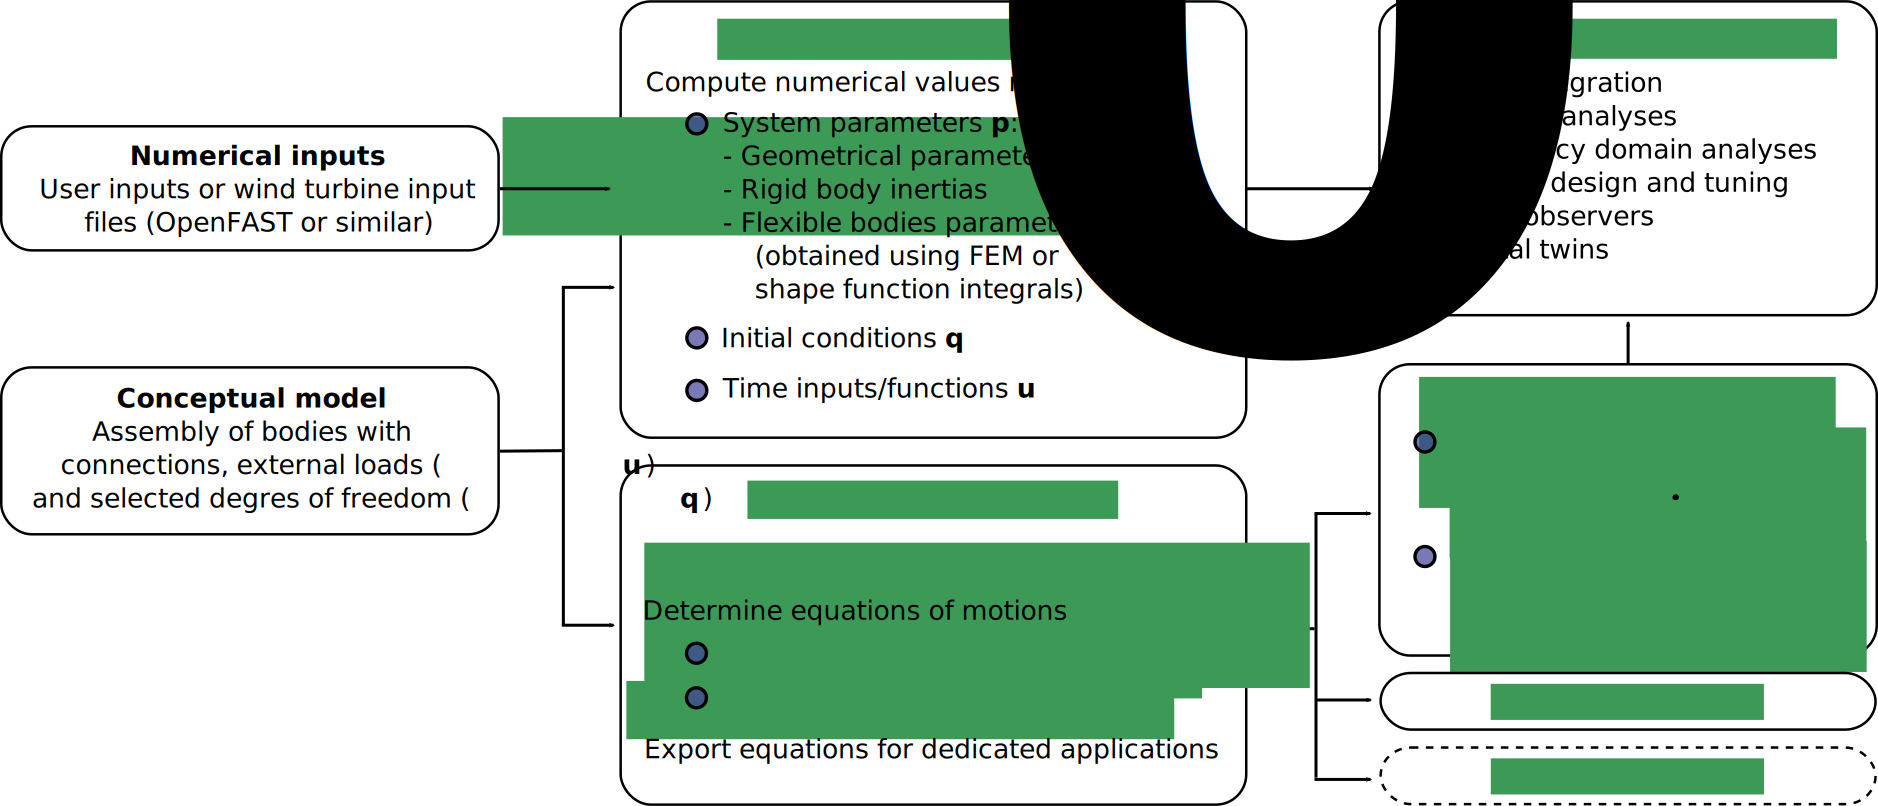
\includegraphics[width=0.89\textwidth]{figs/YAMSWorkflow.pdf}
  \caption{Typical workflow for the usage of the symbolic framework, going from numerical inputs and a conceptual model to numerical packages that can be used for various applications.}\label{fig:YAMSWorkflow}%
\end{figure}
% --------------------------------------------------------------------------------
The symbolic framework takes as input a conceptual model of the structure, which is assembled using one of the three layers previously described. 
The nonlinear and linear equations of motion can be exported to LaTeX and Python-ready scripts for various applications (see \autoref{sec:Applications}).
Using the third layer, as little as three lines of code are required by the user to perform the full step from derivation of the equations, optional linearization, and exportation.
% 
To obtain numerical results from the exported Python code, the user needs to provide the arrays with the degrees of freedom values $\v{q}$ and $\v{\dot{q}}$, their initial conditions, a dictionary with inputs ($\v{u}$) that are functions of time, and a dictionary of parameters ($\v{p}$) containing all the numerical constants such as mass, acceleration of gravity, and geometric parameters.
We implemented various preprocessing tools in YAMS to facilitate the calculation of numerical parameters, typically from a set of OpenFAST input files or by using structural parameters defined by the users. YAMS contains tools to compute the flexible bodies parameters (mass matrix, stiffness matrix, shape integrals) using integrals over the shape functions or using a finite-element beam formulation.
YAMS also contains tools to compute the rigid body inertia of different components of a wind turbine or the full system. Postprocessing tools are also included to readily time-integrate the generated model using numerical values (including initial values).


The source code of YAMS is available on GitHub as a subpackage of the Wind Energy LIBrary, WELIB~\citep{WELIBgithub}.  
The repository contains tests and working examples, including the ones presented in \autoref{sec:WEapplications}.

% The main wrapper for the preprocessing tool is located in the package \texttt{windturbine.py}. The export to the SID format is achieved using the package \texttt{sid.py}, which can compute the flexible body parameters using FEM (package \texttt{beam_beam.py})
% , it relies on the package \texttt{flexibility.py} which computes various flexible body parameters. 
% The finite element package of the repository can be used to generate the SID from beam models such as the ones used for blades and tower.
% \subsection{Maxima implementation}
% \subsection{Misc}
% In some numerical implementation, the partial velocities for each bodies are gathered into matrices $\m{J}_{v,j}$, and $\m{J}_{\omega,j}$, both of dimension $3 \times n_q$.
% Approach
% Misc features




% --------------------------------------------------------------------------------}
% --- Applications 
% --------------------------------------------------------------------------------{
\section{Wind energy applications}
\label{sec:WEapplications}


\subsection{Approach}
In this section, we present different wind energy applications of the symbolic framework. 
We focus on models with at least one flexible body because the rigid body formulation of SymPy has been well verified~\citep{Gede:2013}.
For each example, the equations of motion are given and their results are compared with OpenFAST~\citep{OpenFAST} simulations.
This is readily achieved because our framework can export the equations of motion to Python functions, load input files from an OpenFAST model, and integrate the generated equations using the same conditions as defined in the OpenFAST input files. 
In this article, we do not focus on the modeling of the external loads, but we include them in the equations of motion.
It is the responsibility of the user to define these functions, for instance through aero- or hydro-force models.
For the verification results presented in this section, we only include the gravitational and inertial loading.
In all examples, the National Renewable Energy Laboratory (NREL) 5-MW reference wind turbine~\citep{nrel5mw} is used.
The examples below are provided on the GitHub repository where the YAMS package is provided~\citep{WELIBgithub}.



\subsection{Notations}
We adopt a system of notations where the first letter of a body is used to identify the parameters of that body.
As an example, the tower is represented with the letter T, and the following body parameters are defined: $T$, origin; $M_T$, mass; $L_T$, length; $(J_{x,T}, J_{y,T}, J_{z,T})$, diagonal coefficients of the inertia tensor about the center of gravity and in body coordinates; $\v{r}_{TG}$, vector from body origin to body center of mass, of coordinates $(x_{TG},y_{TG},z_{TG})$ in body coordinates. 
We also define $\theta_t$, the nacelle tilt angle about the $y$ axis; $g$, the acceleration of gravity along $-z$; and $O$, the origin of the global coordinate system.





\subsection{Rotating blade with centrifugal stiffening}
\label{sec:RotatingBlade}
We begin with the study of a flexible blade of length $L_B=R$, rotating at the constant rotational speed $\Omega$.
We use this test case to familiarize the reader with the key concepts of the shape function approach given in \autoref{sec:ShapeFunctionApproachBeam}. 
A sketch of the system is given in \autoref{fig:DynamicsWT1DOF_Blade}.
We start by modeling the blade using a single shape function, assumed to be directed along the $x$-axis (``flapwise''): $\v{\Phi}_1=\Phi \v{e}_x$, where $\v{e}_x$ is the unit vector in the $x$ direction.
% The model can similarly be applied to the edgewise direction and be extended to multiple shape functions containing both flap and edge components (see \cite{branlard:2019flex}).
% --------------------------------------------------------------------------------
\begin{figure}[!htb]
 \centering%
 \def\svgwidth{0.5\columnwidth}%
 \scalebox{0.95}{\import{figs/}{DynamicsWT1DOF_Blade}}%
 \caption{Sketch of a rotating blade with the restoring centrifugal force. Points are indicated in green, degrees of freedom in blue, and loads in orange.}\label{fig:DynamicsWT1DOF_Blade}%
 \end{figure}%
%--------------------------------------------------------------------------------
% --------------------------------------------------------------------------------
The undeflected blade is directed along the radial coordinate $r$ and rotates around the $ x$-axis.
% is either the aerodynamic load in the flapwise direction, 
% We assume that the blade the radial coordinate $r$
We assume that the shape function is known, noted $\Phi(r)$. 
It can be computed as the first flapwise mode of the blade using tools provided in YAMS.
The expression $\Phi(r)=r^3$ is a simple approximation that can be used for hand calculations. 
The aerodynamic force per length in the flapwise direction is noted $p_x(r)$.
% Once a shape function is assumed, the expressions for $M$ and $K$ are directly computed based on the distributed properties of the blade ($EI$ and $m$).
% The loading $p(r)$ is either the aerodynamic load in the flapwise direction, or the aerodynamic load in the edgewise direction (combined with gravitational loads). 
The generalized mass and stiffness are computed based on the mass per length ($m$) and flapwise bending stiffness ($EI_y$) of the blade, according to \autoref{eq:MassMatrixRRBeam}:
\begin{align}
  M_{e}&=\int_0^{R} m(r) \Phi^2(r)\, dr
  \label{eq:MeBlade}
      \\
%       ,\quad
  K_{e}&=\int_0^{R} EI_y(r) \left[\frac{d^2\Phi}{dr^2}(r)\right]^2\, dr
  \label{eq:KeBlade}
\end{align}
The generalized force is obtained from \autoref{eq:GenQBeam}:
\begin{align}
  f_{e}=\int_0^{R} p_x(r,t)\Phi(r)\, dr 
\end{align}


The important consideration for this model is the axial load, $N$.
The main axial load at a radial station $r$ comes from the centrifugal force acting on all the points outboard of the current station:
\begin{align}
    N(r)=\int_r^R m(r') \Omega^2  r' \, dr'
\end{align}
      %\label{eq:}
The geometric stiffness contribution of the axial load is obtained from \autoref{eq:StiffnessAxial} as:
\begin{align}
    K_g(\Omega) = \int_0^R N(r) \left[\frac{d\Phi}{dr} \right]^2  dr  
    = \Omega^2 \int_0^R \int_r^R m(r') r' \, dr'
 \left[\frac{d\Phi}{dr} \right]^2 dr  
 \label{eq:GeomStiffCentri}
\end{align}
%     D_e= 2 \zeta M_e \omega_e
% 
The geometric stiffness, $K_g$, is positive and increases with the square of the rotational speed. 
This restoring effect is referred to as ``centrifugal stiffening.''
In this example, the beam rotates with respect to a fixed support, the influence of gravity is omitted, and no force other than the centrifugal force is assumed in the radial direction 
(the Coriolis force contribution to the radial force is assumed to be negligible for simplicity).
Therefore, the only geometrical stiffness comes from the centrifugal force.
For a wind turbine blade mounted on a flexible support and under the influence of gravity, the different geometrical stiffening terms presented in \autoref{sec:GeometricalStiffness} should be used.
The natural frequency of the blade will increase with the rotational speed as follows:
\begin{align}
   \omega_0(\Omega)=\sqrt{\frac{(K_{e}+ K_g(\Omega))}{M_e}} 
   = \sqrt{ \omega_0^2(0) + \frac{K_g(\Omega)}{M_e} } 
   = \sqrt{ \omega_0^2(0) +  k_\Omega \Omega^2 } 
\end{align}
where $k_\Omega$ is referred to as the ``rise factor'' or ``Southwell coefficient,'' and in our approximation, it is found to be constant: $k_\Omega=K_g(\Omega)/M_e/\Omega^2$.
The coefficient provides the variation of the blade frequency with rotational speed, which is something that is observed on a Campbell diagram when performing stability analyses.
In general, the mode shapes of the blade will also change as a function of the rotational speed, and different shape functions should preferably be used for simulations at different rotational speeds.
The effect is fairly limited, and most OpenFAST practitioners only use one shape function corresponding to the value at rated rotational speed.
Similarly, the Southwell coefficient is a function of the rotational speed, but the variation is negligible as long as the rotational speed is small compared to the natural frequency (e.g., $(\Omega/\omega)^2 \lesssim 5$; see \cite{bielawa:2006:book}), which is the case for wind energy applications.
%     is the , a variable that depends on the blade property.


The treatment for a shape function in the edgewise direction is similar, using $\v{\Phi}_2=\Phi_2 \v{e}_\theta$, 
where $\v{e}_\theta$ is the unit vector in the edgewise direction.
In this case, the centrifugal force also has a component in the tangential direction, $p_{\theta,\text{centri}}(r) = -\Omega^2u_\theta(r) dm(r)$, with $u_\theta=\Phi_2 q$. 
This leads to a generalized force equal to $\int_0^L p_{\theta,\text{centri}} \Phi_2 dr=-\Omega^2 M_{e} q$, or, equivalently, to a stiffness term: $K_{\omega}=-\Omega^2 M_{e}$.
It can be verified that this generalized force corresponds to the contribution $O_{e,11}\omega_x^2$, from $\v{k}_{\omega,e}$, given in \autoref{eq:komegae}.
For an edgewise mode, the frequency therefore evolves as: 
\begin{align}
 \omega_0(\Omega)=\sqrt{\frac{(K_{e}+ K_g(\Omega)+K_\omega(\Omega))}{M_e}}=\sqrt{\omega_0^2(0)+(k_\Omega-1)\Omega^2}
\end{align}
 with $k_\Omega=K_g(\Omega)/M_e/\Omega^2$ and with $K_g$ computed using \autoref{eq:GeomStiffCentri}.



We apply the method to the NREL 5-MW wind turbine using the blade properties and shape functions provided in the ElastoDyn input file. 
We order the degrees of freedom as \nth{1} flap, \nth{1} edge, and \nth{2} flap, assuming no coupling between the shape functions, so that each can be treated individually using the results from this section.
The diagonal coefficients of the mass matrix are $\operatorname{diag}(\m{M}_e) = [9.5e3,\ 1.5e4,\ 5.7e3]$, and for the stiffness matrix they are 
$\operatorname{diag}(\m{K}_e)=[1.7e4,\ 6.7e4,\ 8.7e4]$, computed according to Equations \ref{eq:MeBlade} and \ref{eq:KeBlade}.
The coefficients $k_\Omega$ of each degree of freedom are obtained as $\v{k}_\Omega =[1.7,\ 1.4,\ 5.5]$. We compare the frequencies obtained with the present method against OpenFAST linearization results in \autoref{fig:FrequencyCentrifugalStiffening}.
The simulations were run in vacuum (no gravity, no aerodynamics) and with a cone angle of 0 deg.
% ---------------------------------- FIGURE --------------------------------------
% From script: CentrifugalStiffening.py, folder: C:/Work/_libs/welib/welib/yams/examples_symbol, 2021/05/06
\noindent\begin{figure}[!htb]\centering%
  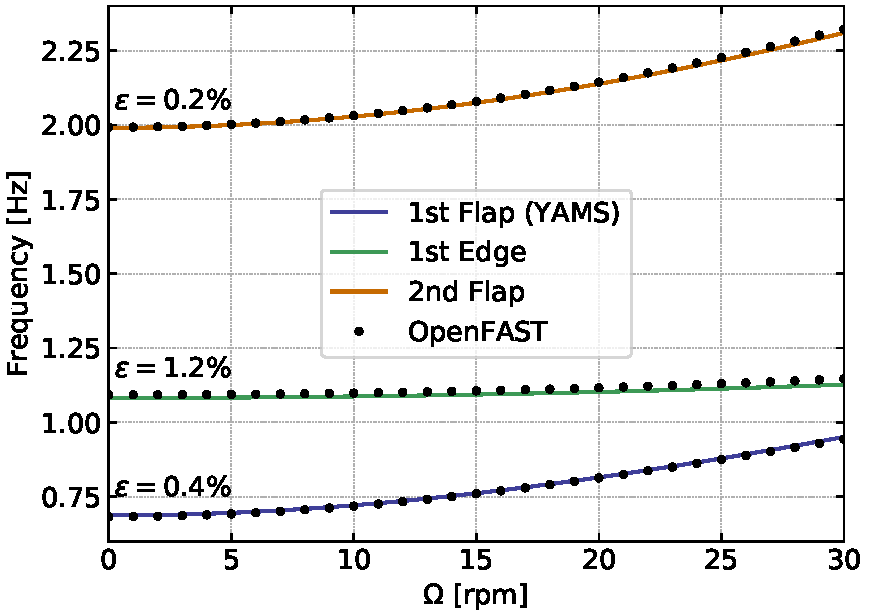
\includegraphics[width=0.48\textwidth]{figs/FrequencyCentrifugalStiffening.pdf}
  \caption{Variation of the natural frequencies of the NREL 5-MW turbine blade with rotational speed. Results from YAMS and OpenFAST, with mean relative error, $\epsilon$, are reported on the figure.}\label{fig:FrequencyCentrifugalStiffening}%
\end{figure}
% --------------------------------------------------------------------------------
Strong agreement is found for the evolution of the different frequencies with the rotational speed.
The stiffening is less pronounced for edgewise modes as a result of the softening introduced by $K_\omega$.

This section focused on the analysis of individual shape functions.
In the general case, multiple shape functions are present and couplings might exist between them (due to the structural twist or nonorthogonality of the shape functions, or if the shape functions have components in multiple directions such as $\v{\Phi_1}=\Phi_{1x}\v{e}_x+\Phi_{1y}\v{e}_y$).
In such a case, the general developments of 
\autoref{sec:FlexibleDefinitions} and 
\autoref{sec:ShapeFunctionApproachBeam} should be used.

% In practice, this effect is limited, and alleviated by using multiple shape functions instead of one.
% The general approach with multiple shape functions is presented in the following sections.
% The general method use multiple shape functions in different directions (e.g., flapwise and edgewise, or fore-aft and side-side). 
% Here, we neglect the fact that $\Phi(r)$ should be adapted for different rotational speeds.




\subsection{Two degrees of freedom model of a land-based or fixed-bottom turbine}
\label{sec:Onshore1DOF}\label{sec:Onshore2DOF}
We consider a system of three bodies: tower (or support structure), nacelle, and rotor.
The system represents a land-based wind turbine or a fixed-bottom offshore wind turbine. 
A sketch of the system is given in \autoref{fig:Onshore3DOF}. 
% --------------------------------------------------------------------------------
\begin{figure}[!htb]%
 \centering%
 \def\svgwidth{0.6\columnwidth}%
 \scalebox{0.9}{\import{figs/}{DynamicsWT3DOF_Onshore}}%
 \caption{Model of a land-based or fixed-bottom wind turbine using one to three degrees of freedom (fore-aft and side-side flexibility of the support structure, and shaft rotation). Points are indicated in green, degrees of freedom in blue, and loads in orange.}\label{fig:Onshore3DOF}%
 \end{figure}%
%--------------------------------------------------------------------------------
The nacelle and rotor blades are rigid bodies, whereas the tower is flexible and represented by one shape function\footnote{
The relevant equations of the shape function approach for a beam are given in \autoref{sec:ShapeFunctionApproachBeam}.} in the fore-aft direction, noted $\v{\Phi}_1=\Phi_1 \v{e}_x$.
%     $\Phi(z) = 1 − \cos(z\pi/L/2)$
For hand calculations and as a first approximation, the first mode shape of a massless beam with a top mass may be used: $\Phi_1(z)=1-\cos(z\pi/L/2)$.
Increased accuracy is obtained when the shape function matches the actual first tower fore-aft bending mode, accounting for the effect of the rotor-nacelle mass and inertia.
    The degrees of freedom are $\v{q}=(q, \psi)$, where $q$ is the generalized (elastic) coordinates in the fore-aft direction and $\psi$ is the azimuthal position.
The slope of the tower shape function at the tower top is a key coupling parameter of the model, noted  $\nu_y$.
When the tower deflects 1 \unit{m} in the $x$ direction, the nacelle rotates by an angle $\nu_y$.
The method assumes that the tower-top point remains along the $x$-axis, neglecting the so-called nonlinear geometric effect.
However, nonlinear geometric effects can be included using geometric stiffening corrections (see  \autoref{sec:GeometricalStiffness} or \cite{branlard:2019flex}).
The aerodynamic thrust and torque are noted $f_a$ and $\tau_a$, respectively, and act at the rotor center (point $R$).
The low-speed shaft generator torque is written as $\tau_g$.
The distributed loads on the tower, $p_x$ (from aerodynamics and hydrodynamics), are projected against the shape function to obtain the generalized forces 
% \begin{align}
  $f_e=\int_0^{L_T} p_x(z,t)\Phi_1(z) dz $.
% \end{align}
The moments of inertia of the rotor in its coordinates are $(J_{x,R}, J_{\oplus,R}, J_{\oplus,R})$.
We note that $M_e, K_e$, and $D_e$ are the generalized mass, stiffness, and damping, respectively, associated with a given shape function
% \begin{align}
$M_e=\int_0^{L_T} m(z) \Phi_1^2(z) dz$
    ,
%       ,\quad
  $K_e=\int_0^{L_T} EI(z) \left[\frac{d^2\Phi_1}{dz^2}(z)\right]^2 dz$
%   ,\quad
,
    $D_e= 2 \zeta M_e \omega_e$.
% \end{align}
where $m(z)$ and $EI(z)$ are the mass per length and bending stiffness of the tower, respectively, and $\omega_e$  and $\zeta$ are the frequency and damping ratio, respectively, associated with the shape function (assuming the shape function approximates a mode shape).
The geometric softening of the tower due to the tower-top mass ($K_{gt}$) and its own weight $(K_{gw}$) is obtained using \autoref{eq:StiffnessAxial}, as $K_g= K_{gt}+K_{gw}$, with :
\begin{align}
  K_{gt}&=- g \int_0^{L_T} (M_{R}+M_N)\left[\frac{d\Phi_1}{dz}(z)\right]^2\, dz
     \\
     % ,\quad
  K_{gw}&=- g \int_0^{L_T} \left[\frac{d\Phi_1}{dz}(z)\right]^2 \left[\int_z^{L_T} m(z')\,dz' \right]  \, dz
      %\label{eq:}
\end{align}
The tower is assumed to be fixed and under no significant vertical external loads and therefore the only geometrical stiffness comes from the gravitational force. For a tower mounted on a moving support (fixed-bottom foundation or floater), additional  geometrical stiffening terms would be present (see \autoref{sec:GeometricalStiffness}).
% 
The shape function frequency is obtained as:
\begin{align}
    \omega_e = \sqrt{(K_e+K_g)/M_e}
\end{align}
% More details on the shape function approach and geometrical stiffening for beams can be found in previous work~\citep{branlard:2019flex}. 
The application of the symbolic framework leads to the following equations of motion (rearranged for interpretability):
\begin{align}
    \begin{bmatrix}
    M_q & 0 \\ 
    0 & J_{x,R} \\ 
    \end{bmatrix}
    \begin{bmatrix}
    \ddot{q}\\
    \ddot{\psi}\\
    \end{bmatrix}
    =
    \begin{bmatrix}
    f_q \\
    \tau_a-\tau_g\\
    \end{bmatrix}
    \label{eq:EOM2DOF}
\end{align}
where:
\begin{align}
M_q = & M_{e} +  M_N + M_R \label{eq:Mq1}\\
     &+ (J_{y N} + J_{\oplus,R} + M_N(x_{NG}^{2} + z_{NG}^{2}) + M_R(x_{NR}^{2} + z_{NR}^{2}) ) \nu_y^{2}  \label{eq:Mq2}\\
     &+2  \left[   (M_N z_{NG} + M_R z_{NR}) \cos{\left(\nu_y q \right)} -(M_N x_{NG} + M_{R} x_{NR})\sin{\left(\nu_y q \right)} \right] \nu_y\label{eq:Mq3}
\end{align}
and
\begin{align}
 f_q &= f_{e} - (K_{e}+K_g) q  - D_{e} \dot{q} \label{eq:Fq1} \\
 &+ g \nu_y \left [ (M_N x_{NG}+M_R x_{NR}) \cos{\left(\nu_y q \right)}
 +                  (M_N z_{NG}+M_R z_{NR}) \sin{\left(\nu_y q \right)} \right]  \label{eq:Fq2}\\
 &+ \nu_y^2 \dot{q}^2\left[
  ( M_N x_{NG} + M_R x_{NR}) \cos{\left(\nu_y q \right)} 
 +( M_N z_{NG} + M_R z_{NR}) \sin{\left(\nu_y q \right)}
 \right]  \label{eq:Fq3} \\
 &+f_a \nu_y ( x_{NR} \sin\theta_t + z_{NR} \cos\theta_t)  \label{eq:Fq4} \\
 &+ f_a \cos{\left(\theta_t + \nu_y q \right)}\label{eq:Fq5} 
\end{align}
Details on the derivations are given in Appendix \ref{sec:Onshore2DOFEq}.
The mass matrix consists of three main contributions:
\autoref{eq:Mq1} represents the elastic mass and the rotor nacelle assembly (RNA) mass,
\autoref{eq:Mq2} is the generalized rotational inertia of the RNA, and
\autoref{eq:Mq3} is the inertial coupling between the tower bending and the rotation of the nacelle.
The forcing terms are identified as follows:
\autoref{eq:Fq1} consists of the elastic load resulting from the external forces on the tower, the elastic and geometric stiffness loads, and the damping load on the tower; 
\autoref{eq:Fq2} is the gravitational load from the RNA, which will contribute to the stiffness of the system; 
\autoref{eq:Fq3} is the centrifugal force of the RNA (``$M \omega^2 r$'' with $\omega=\nu_y \dot{q}$);
\autoref{eq:Fq4} is the generalized torque from the aerodynamic thrust; and  
\autoref{eq:Fq5} is the thrust contribution acting directly along the direction of the shape function degree of freedom (along $x$).
The RNA center of mass plays an important part in the equations (see the terms $(M_N x_{NG}+M_R x_{NR})$ and $(M_N z_{NG}+M_R z_{NR})$). 

The equations of motion given in \autoref{eq:EOM2DOF} can be used to perform time domain simulations of a wind turbine.
It is noted that the two degrees of freedom are only coupled by the aerodynamic loads.
The nonlinear model was used in previous work for time domain simulations and its linear version was used for state estimations~\citep{Branlard:2020twin,Branlard:2020twinOF}.
In this section, we apply the linearized form to compute the natural frequency of the turbine tower fore-aft mode.
The linearized stiffness is obtained by taking the gradient of the forcing with respect to $q$, and using a small angle approximation for $\nu_y$ to the second order:
\begin{align}
K_{q,lin}= (K_{e} + K_g)
- \nu_{y}^{2} g \left(M_N z_{NG} + M_{R} z_{NR} - f_a q \cos\theta_t\right)
+ \nu_{y} f_a \sin\theta_t 
\end{align}
For the NREL 5-MW reference turbine \citep{nrel5mw}, the different numerical values are:
$g=9.807$ \unit{m\cdot s}$^{-2}$,
$\theta_t=5$ \unit{deg},
$x_{NR}=-5.0$ \unit{m},
$z_{NR}= 2.4$ \unit{m},
$L_T=87.6$ \unit{m},
$z_{NG}=1.75$ \unit{m},
$x_{NG}=1.9$ \unit{m},
$M_R= 1.1e5$ \unit{kg},
$J_{x,R}=3.86e7$ \unit{kg\,m}$^2$,
$J_{\oplus,R}=1.92e7$ \unit{kg\,m}$^2$,
$M_N=2.4e5$ \unit{kg},
$J_{y,N} =1.01e6$ \unit{kg\,m}$^2$,
$M_{RNA}=3.5e5$ \unit{kg}.
The first fore-aft shape function of the NREL 5-MW turbine tower and its derivatives are:
\begin{align}
   \Phi_1(z) &= (a_2 \bar{z}^2+ a_3 \bar{z}^3+ a_4 \bar{z}^4+ a_5 \bar{z}^5+ a_6 \bar{z}^6)/(a_2+a_3+a_4+a_5+a_6)\nonumber \\
   \frac{d\Phi_1}{dz}(z) &= \frac{1}{L_T}(2a_2 \bar{z}+ 3a_3 \bar{z}^2+ 4a_4 \bar{z}^3+ 5a_5 \bar{z}^4+ 6a_6 \bar{z}^5)/(a_2+a_3+a_4+a_5+a_6)\label{eq:ShapeFunctionsPoly}  \\  
   \frac{d^2\Phi_1}{dz^2}(z) &= \frac{1}{L_T^2}(2a_2+ 6a_3 \bar{z}+ 12a_4 \bar{z}^2+ 20a_5 \bar{z}^3+ 30a_6 \bar{z}^4)/(a_2+a_3+a_4+a_5+a_6) 
   \nonumber
\end{align}
with $\bar{z}=z/L$, $a_2=0.7004$, $ a_3=2.1963$, $a_4=-5.6202$, $a_5=6.2275$, and $a_6=-2.504$.
The material properties and the shape function are illustrated in \autoref{fig:NREL5MWTower}. 
% ---------------------------------- FIGURE --------------------------------------
% From script: F0T1N0S1_yams_model.py, folder: welib/yams/examples_symbol, 2021/05/04
\noindent\begin{figure}[!htb]\centering%
  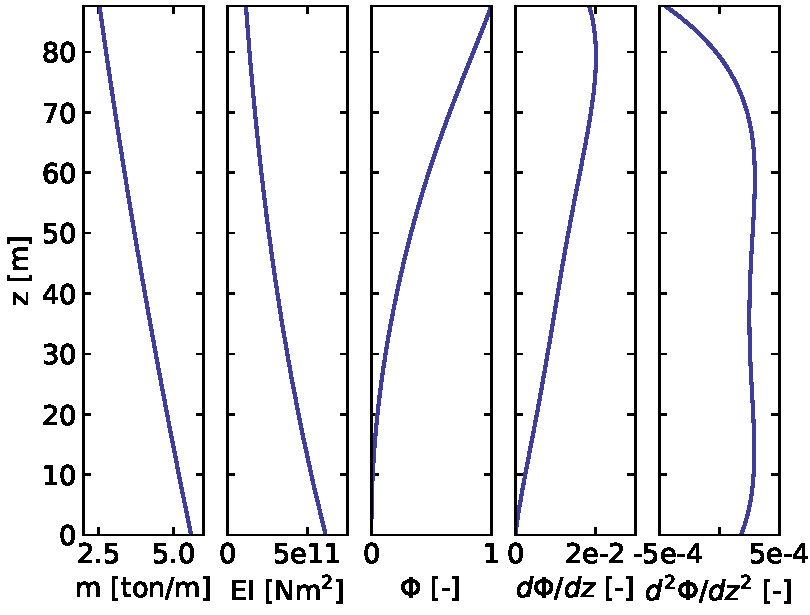
\includegraphics[width=0.49\textwidth]{figs/NREL5MWTower.pdf}
  \caption{Properties of the NREL 5-MW turbine tower: mass per length ($m$), bending stiffness ($EI$), and shape function displacement ($\Phi$), slope ($d\Phi/dz$) and curvature $(d^2\Phi/dz^2)$.}\label{fig:NREL5MWTower}%
\end{figure}
% --------------------------------------------------------------------------------
The scaling of the shape functions given in \autoref{eq:ShapeFunctionsPoly} is important to obtain the correct numerical values for the flexible tower, namely:
$\nu_y=0.0185$,
$M_e=5.4e4$,
$K_e=1.91e6$,
$K_g=  -5.2e4 -1.0e4 = -6.20e4$,
$\omega_e=\sqrt{(K_e+K_g)/M_e}=5.85$ \unit{rad/s}.
% $\zeta=1\%$,
% $D_e= 2 \zeta M_e \omega_e = 6.3e3$.
These numerical values, with $q=0$, lead to:
$M_q = 4.375e5$ and $K_q = 1.849e9$.
The first fore-aft mode of the wind turbine has a natural frequency of $f=\sqrt{K_q/M_q}=0.3272$ \unit{Hz}.
This value was compared with results obtained using OpenFAST linearization.
Both methods are in strong agreement, with differences only arising at the fifth decimal place.








\subsection{Three-degrees-of-freedom model of a land-based or fixed-bottom turbine}
\label{sec:Onshore3DOF}
We consider the same system as the one presented in \autoref{sec:Onshore1DOF}, but 
the tower is now represented by one shape function in both the fore-aft and side-side directions, $\v{\Phi}_1=\Phi_1 \v{e}_x$ and $\v{\Phi}_2=\Phi_2\v{e}_y$.
The degrees of freedom are $\v{q}=(q_1, q_2, \psi)$, where $q_1$ and $q_2$ are the generalized (elastic) coordinates in the fore-aft and side-side directions, respectively, and $\psi$ is the rotor azimuth.
A sketch of the system is given in \autoref{fig:Onshore3DOF}. 


% We consider a system of three bodies: tower (or support structure), nacelle and rotor. The system represents an onshore wind turbine or a fixed-bottom offshore wind turbine. The nacelle and rotors are rigid bodies, whereas the tower is flexible and represented by one shape function in both the fore-aft and side-side directions, $\Phi_1$ and $\Phi_2$. The degrees of freedom are $\v{q}=(q_1, q_2, \psi)$, where $q_1$ and $q_2$ are the generalized (elastic) coordinates in the fore-aft and side-side directions respectively, and $\psi$ is the rotor azimuth. A sketch of the system is given in \autoref{fig:Onshore3DOF}. 
The slopes of the shape functions at the tower top are key coupling parameters of the model, noted $\nu_x$ and $\nu_y$. 
The aerodynamic thrust and torque are noted $f_a$ and $\tau_a$, acting at point $R$.
The distributed loads on the tower, $p_x$ and $p_y$ (from aerodynamics and hydrodynamics), are projected against the shape functions to obtain the generalized forces $f_{e1}=\int \Phi_1 p_x dz$ and  $f_{e2}=\int \Phi_2 p_y dz$. 
The moments of inertia of the rotor in its coordinates are $(J_{x,R}, J_{\oplus,R}, J_{\oplus,R})$.
We note that $\m{M}_e$, $\m{K}_e$, and $\m{D}_e$ are the generalized mass, stiffness, and damping, respectively, associated with a given shape function (e.g., $M_{e11}=\int \Phi_1^2 m(z) dz$, where $m$ is the mass per length of the tower). 
% More details on the shape function approach can be found in previous work~\citep{branlard:2019flex}. 
The application of the symbolic framework leads to the equations of motion given in Appendix \ref{sec:Onshore3DOFEq}.
To simplify the equations and limit their length when printing them in this article, we have applied a first-order small-angle approximation for $\theta_t$, and a second-order approximation for $\nu_x$ and $\nu_y$.
It is observed from \autoref{eq:GMEx1} that a first-order approximation for $\nu_y$ would have removed the influence of the rotor and nacelle $y$-inertia on the generalized mass associated with the tower fore-aft bending. 

We performed a time simulation of the model using both our symbolic framework YAMS and OpenFAST.
The time integration in YAMS currently relies on tools provided in the SciPy package, which implements several time integrators.
A sufficient level of accuracy was obtained using a fourth-order Runge-Kutta method, which is the default method.
Kane's method, which uses a minimal set of coordinates, tends to lead to stiff systems, and it is possible that implicit integrators may be needed for other systems.
We compare the time series obtained using our generated functions with results from the equivalent OpenFAST simulation in \autoref{fig:F0T2N0S1Sim}.
In this simulation, the tower top is initially displaced by $1$ \unit{m} in the $x$ and $y$ directions, and the rotational speed is $5$ \unit{rpm}.
% ---------------------------------- FIGURE --------------------------------------
% From script: F0T2N0S1_yams_model.py, folder: welib\yams\examples_symbol
\noindent\begin{figure}[!htb]\centering%
  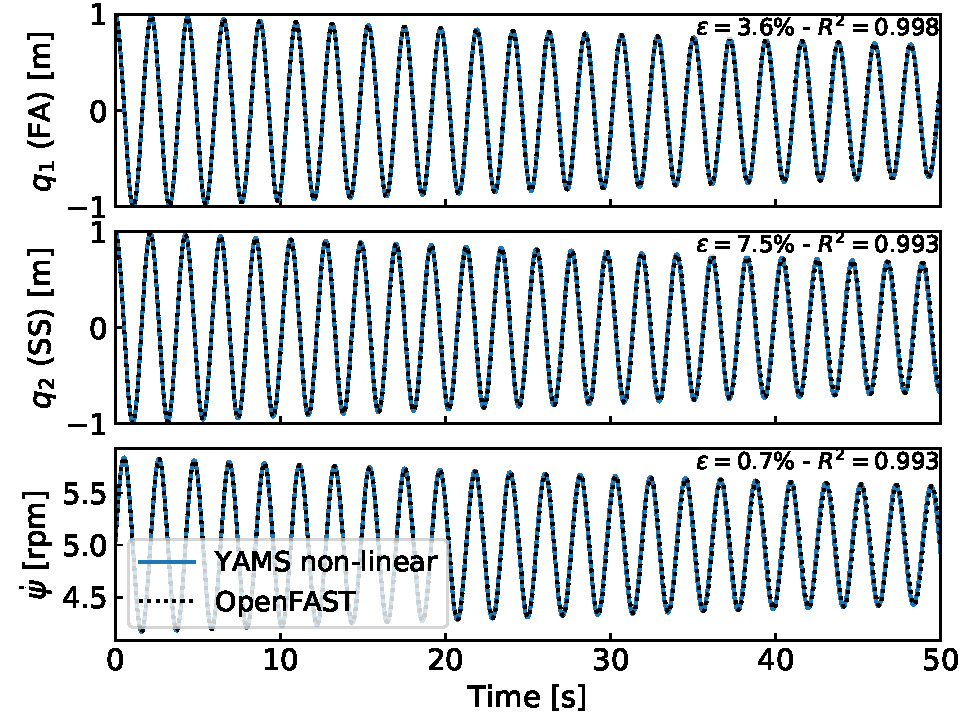
\includegraphics[width=0.49\textwidth]{figs/F0T2N0S1Sim}
  \caption{Free decay results for the land-based/fixed-bottom model using both the symbolic framework (YAMS) and OpenFAST. From top to bottom: tower fore-aft bending, tower side-side bending, and shaft rotational speed.}\label{fig:F0T2N0S1Sim}%
\end{figure}
% --------------------------------------------------------------------------------
We report the mean relative error, $\epsilon$, and the coefficient of determination, $R^2$, on the figure.
We observe that our model is in strong agreement with the OpenFAST simulation.
The differences in the second tower degree of freedom are attributed to 1) the handling of the small-angle approximation, which is different in OpenFAST (using the closest orthonormal matrix; \cite{Jonkman:2009}) and in our formulation (two successive rotations, linearized); 2) the nonlinear geometric corrections that are implemented in OpenFAST, which we have omitted here by only selecting shape function expansion to the zeroth order (see \autoref{sec:AdvancedConsiderations}). 
The variation in azimuthal speed, resulting from the coupling between the gyroscopic loads and the tower bending, is captured well. 








\subsection{Three-degrees-of-freedom model of a floating wind turbine}
\label{sec:Offshore3DOF}
In this example, we demonstrate the applicability of the method for a floating wind turbine.
We model the turbine using three bodies: rigid floater, flexible tower, and rigid RNA (labeled ``N'').
The degrees of freedom selected are: $\v{q}=(x,\phi,q_T)$, where $x$ is the floater surge, $\phi$ is the floater pitch, and $q_T$ is the coordinate associated with a selected fore-aft shape function. 
A sketch of the model is given in \autoref{fig:Offshore3DOF}. 
% --------------------------------------------------------------------------------
\begin{figure}[!htb]%
 \centering%
 \def\svgwidth{0.6\columnwidth}%
 \scalebox{0.9}{\import{figs/}{DynamicsWT3DOF_Offshore}}%
 \caption{Model of a floating wind turbine using three degrees of freedom. Points are indicated in green, degrees of freedom in blue, and loads in orange.}\label{fig:Offshore3DOF}%
 \end{figure}%
%--------------------------------------------------------------------------------
The notations are similar to the ones presented in \autoref{sec:Onshore3DOF}.
Lumped hydrodynamic loads at the floater center of mass are now added.
The model can also be used for a combined tower and floater that is flexible, simply by setting the mass of the floater to zero and including the hydrodynamic loading into the loading $p_x$.
The equations of motion are given in Appendix \ref{sec:Offshore3DOFEq}.
The equations were simplified using a first-order small-angle approximation of $\theta_t$ and $\phi_y$, and a second-order approximation for $\nu_y$.


We performed a numerical simulation of the model generated by YAMS and compared it with OpenFAST for a case with gravitational loads only, starting with $x=0$ \unit{m}, $\phi=2$ \unit{deg}, and $q_T=1$ \unit{m}.
The results are presented in \autoref{fig:F2T1RNASim}.
% ---------------------------------- FIGURE --------------------------------------
% From script: F2T1RNA_yams_model.py, folder: welib\yams\examples_symbolic_wind_turbine, 2021/01/13
\noindent\begin{figure}[!htb]\centering%
  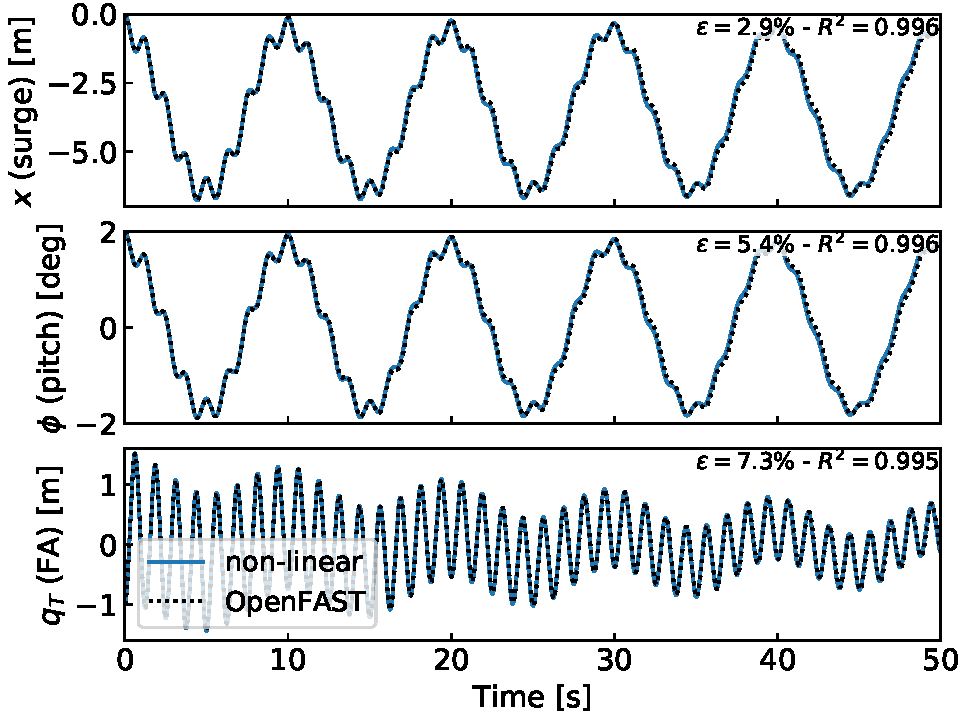
\includegraphics[width=0.49\textwidth]{figs/F2T1RNASim}
  \caption{Free-decay results for the floating wind turbine model using YAMS and OpenFAST. From top to bottom: surge, pitch, and tower fore-aft bending.}\label{fig:F2T1RNASim}%
\end{figure}
% --------------------------------------------------------------------------------
We observe again that the results from the two models correlate to a high degree.

We also compared the linearized version of both models.
The symbolic framework can generate the linearized mass, stiffness, and damping matrices, as described in \autoref{sec:linearization}.
The matrices are then combined into a state matrix and compared with the state matrices written by the OpenFAST linearization feature.
The eigenvalue analysis of the YAMS state matrix returned a pitch and fore-aft frequencies of $0.099$ \unit{Hz} and $0.799$ \unit{Hz}, respectively, whereas OpenFAST returned $0.095$ \unit{Hz} and $0.795$ \unit{Hz}. The $4\%$ error in the pitch frequency appears reasonable in view of the approximations used.


% \subsection{Model with blade flexibility}


% \subsection{Many DOFs}




% --------------------------------------------------------------------------------}
% --- Discussions 
% --------------------------------------------------------------------------------{
\section{Discussions}


\subsection{Applications and advantages of the method}
\label{sec:Applications}\label{sec:Advantages}
The implementation of the symbolic YAMS library was originally motivated by the need to obtain a simple linearized model of a floating wind turbine for frequency domain simulations.
There are multiple potential applications of the framework:
\begin{itemize}
\item The generated equations can be used in time domain simulation tools.
The equations can be readily exported to different programming languages (C, FORTRAN, or Python)  providing computationally efficient tools, particularly because the method generates compact and minimal equations.
% Many automatic code generation libraries also support further optimization by eliminating the repeated calculation of reused terms and terms that only comprise constant parameters.
This is in contrast to most other multibody codes, in which many terms are calculated as matrix equations and through successive function calls.
Further, the symbolic framework allows us to generate optimized code, in which common terms and factors are computed once and stored in temporary variables for reuse in the different expressions.
%
In our examples, time domain simulations were observed to be 2 orders of magnitude faster when using the automatically generated code in Python compared to OpenFAST simulations that rely on a compiled language. 
%
Using such a framework can be considered in the future to replace the existing ElastoDyn module of OpenFAST.
It can also be applied to unusual configurations such as multirotor or vertical-axis turbine concepts. 
%
Dedicated code can be generated for specific applications for increased performance.
For instance, implicit integrators with iterative Newton-Raphson-like solvers benefit from the possibility of generating exact and efficient Jacobians along with the equations of motion.
% \item The generated code can be taylored to use solvers from standard libraries or custom integrators or it can be generated as the bare differential equations for use in a co-simulation environment, e.g. as an S-function in MATLAB/Simulink.

% For complex expressions this is usually much more that modern compilers can do. A similar approach can factor out subexpressions that consist of only parameters. These subexpressions can be precomputed leading to even better run-time performance.

\item The shape function approach introduces a separation of space and time early on in the development of the nonlinear equations, and applies low order polynomial (usually linear or quadratic) approximations to eliminate high-order terms (see e.g. Table 1 of \cite{Wallrapp:1994}). Because of this, the linearization of the nonlinear equations is straightforward, but the linear solutions will only be valid in the neighborhood of the operating point where they are evaluated. 
The approximations introduced by the method may imply that non-linearities are not well captured, which is the why the models are labeled as ``mid-fidelity'' throughout this article. 
Advanced methods to obtain high-fidelity reduced-order (linear or nonlinear) models from nonlinear dynamic systems are beyond the scope of this work, see, e.g.
\cite{Steindl:2001, Mignolet:2013, Benner:2015}.


%     \item The wall time is two order of magnitude faster despite using Python
\item The generation of linearized models has a wide range of applications, such as linear time domain simulations, controller design and tuning, frequency domain analyses, stability analyses, state observers, or digital twins.
The symbolic approach is severalfold faster than alternative approaches because it can be evaluated for all operating points at once, whereas other methods (e.g., OpenFAST, HAWCStab2) require multiple linearization calls.
% Also, model order reduction of the linearized models is not necessary, because our models already start out with a reduced number of degrees of freedom and modes for the flexible bodies.

\item Analytical linearization with respect to parameters is directly obtained using our tool, which can be used for sensitivity analyses, parameter studies, optimizations, integrated design approaches, and controls co-design (e.g., using methods such as linear-matrix-inequality-based designs) \citep{Poschke:2020}.  Nonanalytical approaches require numerous linearizations and evaluations at various operating points \citep{Jonkman:2022lin}.

\item In addition to the nonlinear or linear equations of motion in minimal coordinates, the equations for the constraint forces or any auxiliary kinematic variable can also be generated efficiently by inserting unknown virtual displacements in the equations (see Appendix \ref{sec:PartialLoads} for an alternative approach). 
The position of all bodies in local or global coordinates can be recovered from the minimal coordinates and, in combination with the flexible code generation, be used to output data (e.g., for 3D animations of the turbine). 

\item Analytical gradients of the equations can be computed and used in optimizations,
nonlinear model predictive control, or moving horizon estimation.
    External loads that cannot be expressed analytically can be defined as generic functions of the structural degrees of freedom, inputs, and parameters.
    After the code generation, the user can link a numerical implementation of the function and its numerical gradients to be able to use a mix of analytical and numerical gradients.

\item Another advantage of the presented method is the possibility to quickly generate models with different levels of detail, ensuring consistency between the different levels of fidelity.
This is in contrast to other more heuristic modeling approaches in which parameters often have to be retuned for each added degree of freedom.

\item The method provides useful insights and can be used as an educational tool: simple models of a system with few degrees of freedom can readily be obtained, studied, and compared to hand-based calculation.
% The flexibility of the presented approach regarding the variation of model properties and the presentation of the resulting equations make the framework ideal for educational purposes.
% The effects of different aspects can be studied and analysed; using numerical methods, symbolic analysis or by plain reading of well formated LaTeX equations.
% The whole processing chain of the equations is accessible and therefore transparent. 
% Resulting terms in the minimal equations of motion can be traced back to their physical meaning. 
% The difference it makes to include some or other detail becomes directly apparent.
% \item 
%  generation of dedicated code (for standalone simulations, state observers or digital twins). 
% Further processing by specialized tools, e.g. for the generation of high performance NMPC code
% such as acados (Verschueren et al., 2018)
\end{itemize}


% \subsection{Advantage of using a symbolic framework}
% \label{sec:Advantages}
% Most advantages have already been discussed in \autoref{sec:Applications}, namely: the wide range of applications and the potential gain in computational time.
% Additionally, the method can provide useful insights and be used as an educational tool: simple models of a system with few degrees of freedom can readily be obtained, studied, and compared to hand-based calculation.

% \begin{itemize}
%     \item linearization, evaluations
%     \item Using a symbolic framework offers great advantages in terms of speed and may allow for features that are not available in currently available tools.
%     \item applications: frequency domain, controller design, stability analyses, estimations
%     \item educational
% \end{itemize}

\subsection{Advanced consideration}
\label{sec:AdvancedConsiderations}

Section \ref{sec:method} addressed the systematic derivation of the equations of motion for an assembly of rigid or flexible bodies.
    Some advanced aspects of the method are discussed here:
\begin{itemize}
    \item
%         The expression of the displacement field $\v{u}$ in terms of a superposition of shape function is typically done using a zeroth or first-order expansion. 
The different terms involved in the equations of motion of flexible bodies can be decomposed using shape integrals (see Appendix \ref{sec:TaylorExpansionShapeIntegrals}).
% 
% or not.  We discuss these formulations in \autoref{sec:TaylorExpansion}.
Our framework readily supports this optional decomposition: it is the responsibility of the user to provide the terms and values of the expansion when numerical evaluation is to occur.

    \item The definition of geometric stiffening requires attention in the general case.
    It is accounted for by the term $\v{k}_\sigma$, presented in \autoref{sec:FlexibleDefinitions}.
    We discuss geometric stiffening in more detail in \autoref{sec:GeometricalStiffness}.
%     A general account of the effect for an arbitrary geometry can be found in \citep{Schwertassek:book, Wallrapp:1991}. A, simplified expressions are given for beams in \autoref{sec:ShapeFunctionApproachBeam}.

    \item The treatment of external loads was not addressed in detail in this article because the loads are application-specific (aerodynamics, hydrodynamics, etc.).
    The framework can accept external loads as arbitrary functions of multiple variables or as analytical expressions.
    In the former case, the user will have to provide an implementation of the function during the execution.

    \item Even though the equations of motion are void of constraint forces, the values of these forces can be recovered.
    They can be expressed as functions of the external forces and the states of the system.
    It is not necessary to compute them by iteratively solving constraint equations.
    %They can be derived using this framework, by introducing a virtual degree of freedom allowing motion

    \item The framework can easily include rheonomous constraints---for instance, for the pitch angle---without having to supply a dedicated torque.
    Pitch speed and accelerations can be directly introduced into the mechanical system if they are provided by a generic second-order pitch actuator model.
\end{itemize}




\subsection{Limitations}
In spite of the advantages listed in \autoref{sec:Advantages}, the symbolic procedure presented in this work has some potential limitations.
We are identifying two in this section.
First, constraints and closed loops have currently not been added to the framework.
The SymPy mechanics package supports additional constraint equations within Kane's method.
We therefore hope that this limitation can be lifted in the future.
Second, large problems may challenge a symbolic calculation package: memory impact, calculation time, simplification times, and size of expressions may become significant.
Some of these issues may be alleviated by introducing intermediate variables that are only substituted for in the numerical implementation or by using a recursive formulation of the solution procedure~\citep{branlard:2019flex}.
% Third, the method of minimal coordinates leads to compact and highly nonlinear equations of motion.



% --------------------------------------------------------------------------------}
% --- Conclusions 
% --------------------------------------------------------------------------------{
\conclusions

We presented a symbolic framework to obtain the linear and nonlinear equations of motion of a multibody system made of rigid bodies, flexible bodies, and kinematic joints.
Our approach is based on Kane's method and a nonlinear shape function representation of flexible bodies.
We provided different wind energy examples and verified the results against OpenFAST simulations.
The framework can readily provide models suitable to a wide range of applications with competitive computational times.
The framework is open source, and the examples presented are available in the repository.
Future work will focus on applying the framework to dedicated research projects, with more complex systems, and potentially extend the framework to account for closed-loop systems and arbitrary constraints.






\authorcontribution{
Both authors exchanged over the last two years about the implementation of such a framework and its application to wind energy. 
EB wrote a Python implementation and JG wrote a Maxima implementation.  EB wrote the main corpus of the article, with feedback and contributions from JG.}

\competinginterests{No competing interests are present.} %% this section is mandatory even if you declare that no competing interests are present


\codeavailability{
    A Zenodo link will be created for \url{https://github.com/ebranlard/yams}.
    The examples given in this articles are found in the folder \texttt{welib/yams/papers} of the repository.
%     \todoEmmanuel{Create a Zenodo link for welib/yams
%     \url{https://github.com/ebranlard/yams}. No rush}
% 
%     \todoJens{A Zenodo link for CADyn (No rush on that, we can wait for the article to be fully accepted..}
%     \todoEmmanuel{Mention where the examples are in the repo}
} %% use this section when having only software code available

% \acknowledgements{
% This work was authored by staff from the National Renewable Energy Laboratory, operated by Alliance for Sustainable Energy, LLC, for the US Department of Energy (DOE) under contract no. DE-AC36-08GO28308. Funding provided by the US Department of Energy Office of Energy Efficiency and Renewable Energy Wind Energy Technologies Office. The views expressed in the article do not necessarily represent the views of the DOE or the US Government. The US Government retains and the publisher, by accepting the article for publication, acknowledges that the US Government retains a nonexclusive, paid-up, irrevocable, worldwide license to publish or reproduce the published form of this work, or allow others to do so, for US Government purposes.
% }
% 

% \disclaimer{TEXT} %% optional section
%% REFERENCES
%% The reference list is compiled as follows:
\acknowledgements{
This work was authored in part by the National Renewable Energy Laboratory, operated by Alliance for Sustainable Energy, LLC, for the U.S. Department of Energy (DOE) under Contract No. DE-AC36-08GO28308. Funding provided by U.S. Department of Energy Office of Energy Efficiency and Renewable Energy Wind Energy Technologies Office. 
The views expressed in the article do not necessarily represent the views of the DOE or the U.S. Government. The U.S. Government retains and the publisher, by accepting the article for publication, acknowledges that the U.S. Government retains a nonexclusive, paid-up, irrevocable, worldwide license to publish or reproduce the published form of this work, or allow others to do so, for U.S. Government purposes. 
}

\financialsupport{
This work was funded under the Technology Commercialization Fund Project, supported by the DOE's Wind Energy Technologies Office. }


\appendix


% --------------------------------------------------------------------------------}
% ---  
% --------------------------------------------------------------------------------{
\section{Equations for a flexible body and shape integrals}
\label{sec:FlexibleDefinitions}
% \subsection{General equations}
In this section, we detail the equations of motion of a flexible body. 
The reader is referred to the following references for a complete treatment of the equations of motion: \cite{shabana:book}, \cite{Schwertassek:book}, and \cite{Wallrapp:1994}.
% 
% TODO TODO
%     The different terms involved can be expressed as a linear superposition of constant terms, referred to as shape integrals, and time-dependent variables that are function of the degrees of freedoms.
% The shape integrals can be numerically evaluated for beams and beam-based finite-element-models using the tools provided by our framework and gathered into the SID format defined by Wallrapp~\cite{Wallrapp:1993}.
% 
% 
The subscript $i$, indicating the body index, is dropped.
All quantities (vectors and matrices) are expressed in the body frame of reference; therefore, the prime notation is also dropped in this section.
The number of flexible shape functions associated with the body is $n_e$, the flexible degrees of freedom are $\v{q}_e$, and the shape functions are gathered into a matrix $\m{\Phi}$ of size $(3\times n_e)$. 
The equations of motion, given in \autoref{eq:EOMFlexibleBody}, are repeated below:
\begin{align}
    \begin{bmatrix}
       \M_{xx}    & \M_{x \theta} & \M_{ x e } \\
                   & \M_{\theta \theta}   & \M_{\theta e}   \\
       \text{sym.} &            & \M_{e e}  \\
    \end{bmatrix}
    \begin{bmatrix}
      \v{a}_i \\
      \v{\dot{\omega}}i \\
      \v{\ddot{q}}_{e} \\
    \end{bmatrix}
      +
    \begin{bmatrix}
      \v{k}_{\omega, x} \\
      \v{k}_{\omega, \theta} \\
      \v{k}_{\omega, e} \\
    \end{bmatrix}
      +
    \begin{bmatrix}
      0 \\
      0 \\
      \v{k}_{e}\\
    \end{bmatrix}
      =
    \begin{bmatrix}
      \v{f}_{x} \\
      \v{f}_{\theta} \\
      \v{f}_{e}\\
    \end{bmatrix}
    \label{eq:EOMFlexibleBodyRepeated}
\end{align}
The different terms of the mass matrix are obtained as follows:
\begin{align}
   \M_{xx}           & =  \int \m{I}_3 \,\dm = M \m{I}_3  \qquad (3\times3)
       \\
   \M_{x\theta}      & = -\int \stil_P \,\dm          = -M \m{\tilde{s}}_{CM}    \qquad (3\times3)
      \label{eq:MMxt} \\
   \M_{\theta\theta} & = -\int \stil_P \stil_P \,\dm = \v{J}   \qquad (3\times 3) 
   \\
   \M_{\theta e}     & =  \int \stil_P \m{\Phi} \,\dm=\m{C}_r^T  \qquad (3\times n_e)
   \\
   \M_{x e}          & =  \int \m{\Phi} \,\dm =\m{C}_t^T  \qquad (3 \times n_e)
      \label{eq:MMxe} \\
   \M_{e e}          & =  \int {\m{\Phi}}^T \m{\Phi} \,\dm  \qquad (n_e \times n_e)
    \label{eq:MMFlexible}
\end{align}
The integrals are volume integrals over the volume of the body (for beams, they reduce to line integrals).
    The notation $[\tilde{\ \ }]$ represents the skew symmetric matrix.
    $M$ is the mass of the body. 
The vector $\v{s}_{CM}$ is the vector from the origin of the body to undeflected center or mass (CM) of the body.
The notations $\m{C}_t$ ($n_e\times 3$) and $\m{C}_r$ ($n_e\times 3$) are introduced to match Wallrapp's notations.
The vector $\s_{P}$ is the vector from the origin of the body to a deflected point of the body of elementary mass $\dm$.
The undeflected position of this point is written as $\s_{P_0}$ and the displacement field $\v{u}$, such that:  $\s_{P}=\s_{P_0} + \v{u}$.
Typically, the displacement field is given by $\v{u}=\m{\Phi} \v{q}_e$, but a higher-order expansion can also be introduced (see \cite{Wallrapp:1994}  and Appendix \ref{sec:TaylorExpansionDisplacement}).
% For a zeroth order expansion of .
% First-order expansions need the introduction of an additional notation:  $\v{u}=\m{\Phi}_u(\v{q}_e) \v{q}_e$ (see \autoref{sec:AdvancedConsiderations} and .
Wallrapp also includes the elementary mass moment of inertia, which results in additional terms in the integrals (see \cite{Wallrapp:1994}).
Such contributions are relevant, for instance, when considering the torsion of a beam (see \cite{branlard:2019flex}).
The block matrices $\M_{xx}$, $\M_{xe}$, and $\M_{ee}$ do not depend on the deformation of the body and are therefore constant.
The other terms are functions of $\v{q}_e$.
They may be expressed as linear combinations of constant integrals (see Appendix \ref{sec:TaylorExpansionShapeIntegrals}).

% See flexibility.py (GMBeam) or yams_sympy.py (BodyQuadraticForce)
The quadratic velocity terms, $\v{k}_\omega$,  are given as:
\begin{align}
  % ---- komega_x
  \v{k}_{\omega, x}       & = 2\v{\tilde{\omega}}  \v{C}_t^T \v{\dot{q}}_e
      + 
M\v{\tilde{\omega}} 
 \v{\tilde{\omega}} 
\v{s}_{CM}
 \qquad (3\times 1)
 % NOTE:  om_til * skew(self.mdCM.eval(q)) * omega
 % OR     om_til * om_til * self.mdCM.eval(q)
 % JENS convention of MdCM is opposite Wallrapp
  \\
  % ---- komega_theta
  \v{k}_{\omega, \theta}  & = \v{\tilde{\omega}}\M_{\theta\theta}\v{\omega}         
   +\left[\sum\limits_{j=1..n_e}  \v{G}_{r,j} \dot{q}_{e,j}\right] \v{\omega}
 \qquad (3\times 1)
  \\
  % ---- komega_e
  \v{k}_{\omega, e}   & =  \left[  \v{\omega}^T \m{O}_{e,j}\v{\omega}\right]_{j=1..n_e} 
  + 
    \left[\sum\limits_{j=1..n_e}   \m{G}_{e,j} \dot{q}_{e,j}\right] \v{\omega}
 \qquad (n_e\times 1)
 \label{eq:komegae}
%   k_omega[6:6+nq,0] = self.Oe.eval(q) * omega_q
%   for k in np.arange(nq):
%       k_omega[6:6+nq,0] += self.Ge[k].eval(q) * qd[k] * omega
%             Oe6[j][0] = Oe[j][0,0]
%             Oe6[j][1] = Oe[j][1,1]
%             Oe6[j][2] = Oe[j][2,2]
%             Oe6[j][3] = Oe[j][0,1] + Oe[j][1,0]
%             Oe6[j][4] = Oe[j][1,2] + Oe[j][2,1]
%             Oe6[j][5] = Oe[j][0,2] + Oe[j][2,0]
\end{align}
where
\begin{align}
    \m{G}_{r,j} &=  -2 \int   \stil_P \m{\tilde{\Phi}}_j \,\dm \qquad (3\times 3) 
%      # --- Gr_j = - 2*\int [~s] [~Phi_j]
        \\
    \m{O}_{e,j} &=  \int  \m{\tilde{\Phi}}_j \stil_P\,\dm = -\frac{1}{2}  \m{G}_{r,j}^T  \qquad (3\times 3) 
    \\
    \m{G}_{e,j} &=  -2 \int  \m{\Phi}^T \m{\tilde{\Phi}}_j \,\dm \qquad (n_e\times 3) 
\end{align}
The first term of \autoref{eq:komegae} is obtained by vertically stacking the contribution of each shape function. 
In the standard input data format, this term is reshaped as the product $\m{O_e}\v{\Omega}$, where: 
\begin{align}
  \m{O}_e &= \left[O_{e,j,11},\ O_{e,j,22},\  O_{e,j,33},\ O_{e,j,12}+O_{e,j,21},\ O_{e,j,23}+O_{e,j,32},\ O_{e,j,13}+O_{e,j,31}\right]_{j=1..n_e}  \qquad (n_e\times 6)
       \\
 \v{\Omega} &=  \left[\omega_x^2,\ \omega_y^2,\ \omega_z^2,\ \omega_x \omega_y,\ \omega_y \omega_z,\ \omega_x \omega_z \right] \qquad (6\times 1)
      %\label{eq:}
%         omega_q = Matrix([ox**2, oy**2,oz**2, ox*oy, oy*oz, ox*oz]).reshape(6,1)
\end{align}
% 
The body elastic forces are given by:
\begin{align}
  \v{k}_e =  \v{k}_\sigma + \m{K}_e \v{q}_e  + \m{D}_e \v{\dot{q}}_e     %\label{eq:}
\end{align}
where $\m{K}_e$ and $\m{D}_e$ are the elastic stiffness and damping matrices, and $\v{k}_\sigma$ represents geometric stiffening terms (see \autoref{sec:GeometricalStiffness}). 
%     For a bending beam the element $K_{e,ij}$ is the integral over the length of the beam ($L$) of the bending stiffness ($EI$) multiplied by the curvatures of shape functions  $i$ and $j$:
% \begin{align}
%    K_{e,ij} = \int_{0}^L \left[EI_z \frac{d^2 \Phi_{i,y}}{dx^2} \frac{d^2 \Phi_{j,y}}{dx^2} + EI_y \frac{d^2 \Phi_{i,z}}{dx^2} \frac{d^2 \Phi_{j,z}}{dx^2}\right] \, dx
% \end{align}
The elastic damping forces are often given as stiffness proportional damping.
For more details, see \cite{Wallrapp:1994}, and for more examples with elastic beams, see \cite{branlard:2019flex}.
% 
The external loads can be assumed to consist of distributed volume forces, $\v{p}$ (in practice they are primarily surface forces or line forces), and a gravitational acceleration field, $\v{g}$.
The components of the external loads  in  \autoref{eq:EOMFlexibleBodyRepeated} are then obtained by integration over the whole body:
\begin{align}
    \v{f}_x&=\int \v{p} \, dV
        + \m{M}_{xx}\v{g}
        \qquad (3\times 1)
            \label{eq:genQgeneral}
    \\
    \v{f}_\theta&=\int \v{s}_P\times\v{p} \, dV
        + \m{M}_{\theta x}\v{g}
        \qquad (3\times 1)
    \\
    \v{f}_e&=\int {\m{\Phi}}^T\, \v{p} \, dV
        + \m{M}_{e x}\v{g}
        \qquad (n_e\times 1)
\end{align}



%         # --- Ge_j = - 2*\int [Phi]^t  [~Phi_j]
%         # [Phi]: 3xnf
%         Ge = np.zeros((nf,nf,3))
%         for j in range(nf):
%             for k in range(nf):
%                 Ge[j][k,0] = -2*( trapzs(U[k][1,:]*U[j][2,:]*m) - trapzs(U[k][2,:]*U[j][1,:]*m))
%                 Ge[j][k,1] = -2*(-trapzs(U[k][0,:]*U[j][2,:]*m) + trapzs(U[k][2,:]*U[j][0,:]*m))
%                 Ge[j][k,2] = -2*( trapzs(U[k][0,:]*U[j][1,:]*m) - trapzs(U[k][1,:]*U[j][0,:]*m))

% 
%         # --- Oe_j = \int [~Phi_j] [~s] = { \int [~s] [~Phi_j] }^t = -1/2 *(Gr_j)^t
%         Oe = np.zeros((nf,3,3))
%         Oe6= np.zeros((nf,6))
% 
%         for j in range(nf):
%             sxx = trapzs(s_G[0,:]*U[j][0,:]*m)
%             sxy = trapzs(s_G[0,:]*U[j][1,:]*m)
%             sxz = trapzs(s_G[0,:]*U[j][2,:]*m)
%             syx = trapzs(s_G[1,:]*U[j][0,:]*m)
%             syy = trapzs(s_G[1,:]*U[j][1,:]*m)
%             syz = trapzs(s_G[1,:]*U[j][2,:]*m)
%             szx = trapzs(s_G[2,:]*U[j][0,:]*m)
%             szy = trapzs(s_G[2,:]*U[j][1,:]*m)
%             szz = trapzs(s_G[2,:]*U[j][2,:]*m)
%             Gr[j][0,:] = 2*np.array([ syy+szz, -syx  , -szx     ])
%             Gr[j][1,:] = 2*np.array([ -sxy   ,sxx+szz, -szy     ])
%             Gr[j][2,:] = 2*np.array([ -sxz   , -syz  , sxx+syy  ])



%         # --- Gr_j = - 2*\int [~s] [~Phi_j]
%         Gr = np.zeros((nf,3,3))
% 
%         # --- Oe_j = \int [~Phi_j] [~s] = { \int [~s] [~Phi_j] }^t = -1/2 *(Gr_j)^t



%     \label{eq:MFlexible}
% \end{xalignat}
% \begin{xalignat}{3}
%     \M_{xx}'           &=  \int \m{I}_3 \,\dm = M \m{I}_3
%     &
%     \M_{x\theta}'      &= -\int \stil_P' \,\dm  
%     &
%     \M_{x g}'          &=  \int \m{\Phi}' \,\dm 
%     \nonumber\\
%     \M_{\theta\theta}' &= -\int \stil_P' \stil_P' \,\dm 
%     &
%     \M_{\theta g}'     &=  \int \stil_P' \m{\Phi}' \,\dm 
%     &
%     \M_{g g}'          &=  \int {\m{\Phi}'}^t \m{\Phi}' \,\dm
%     \label{eq:MFlexible}
% \end{xalignat}



% --------------------------------------------------------------------------------}
% ---  BEAM
% --------------------------------------------------------------------------------{
\section{Application of the shape function approach to an isolated beam}
\label{sec:ShapeFunctionApproachBeam}
In this section, we illustrate how the elastic equations of \autoref{sec:FlexibleDefinitions} can be applied to an isolated beam. 
Examples of applications are further given in \autoref{sec:RotatingBlade} and \autoref{sec:Onshore2DOF}.
We consider a beam directed along the $z$-axis and bending in the $x$ and $y$ directions.
Expressions are written in the coordinate system of the beam and primes are dropped in this section.
The beam properties are the following: length, $L$, mass per length, $m$, and bending stiffness, $EI_x$ and $EI_y$.
%     and $EI_y$, elongation stiffness $EA$, and torsional stiffness $GK_t$. 
We assume that the displacement field is such that the shape functions are functions of $z$ only:
% \begin{align}
  $  \v{u}(z,t) = \sum_{i=1}^{n_e} \v{\Phi}_i(z) q_{e,i}(t)$.
% \end{align}
We also assume that the shape functions satisfy at least the geometric boundary conditions. 
%     Because the dynamic boundary conditions may not be satisfied by the $\v{\Phi}_i$, we will use an energy formulation to derive the equations of motion.
% 
The kinetic energy of the beam is $T= \frac{1}{2}\int_0^L m \dot{u}^2 dz=\frac{1}{2}\sum_i\sum_j M_{e,ij} \dot{q}_{e,j}\dot{q}_{e,i}$.
% , where the velocity of each point of the beam is obtained as $\dot{u}(z) = \sum_{i=1}^n \v{\Phi}_i(z) \dot{q}_i(t)$. After development, the kinetic energy is found to be $T=\frac{1}{2}\sum_i\sum_j M_{ij} \dot{q}_j\dot{q}_i
where $M_{e,ij}$ is (see \autoref{eq:MMFlexible}):
\begin{align}
  M_{e,ij} = \int_0^L m(z)\, \v{\Phi}_i(z)\cdot \v{\Phi}_j(z)\,dz 
      ,\quad i,j=1,\ldots n_e
      \label{eq:MassMatrixRRBeam}
\end{align}
\autoref{eq:MassMatrixRRBeam} involves a scalar product of the shape functions at each spanwise position.
    Integrals over the moment of inertia can be used to account for torsion (see \cite{branlard:2019flex}).
The potential energy (strain energy) of the beam, is obtained as $V=\frac{1}{2} \sum_i \sum_j K_{e,ij}q_{e,i} q_{e,j}$, where $K_{e,ij}$ are the elements of the stiffness matrix, which, under the assumption of small deformations, are given by:
\begin{align}
%   K_{e,ij} = \int_0^L \left[EI_x(z) \kappa_{i,x}(z)\kappa_{j,x}(z)  + EI_y \kappa_{i,y}\kappa_{j,y}\right] \,dz 
%       \\
%   K_{ij} = \int_0^L\left[ EI_x \kappa_{i,x}\kappa_{j,x} + EI_y \kappa_{i,y}\kappa_{j,y} + EA \kappa_{i,z}\kappa_{j,z} +  GK_t \kappa_{i,\theta}\kappa_{j,\theta}  \right]\,dz 
    K_{e,ij} = \int_{0}^L \left[EI_y \frac{d^2 \Phi_{i,x}}{dz^2} \frac{d^2 \Phi_{j,x}}{dz^2} + EI_x \frac{d^2 \Phi_{i,y}}{dz^2} \frac{d^2 \Phi_{j,y}}{dz^2}\right] \, dz
      ,\quad i,j=1,\ldots n_e
      \label{eq:stiffnessMatrixRRBeam}
\end{align}
% where $\kappa_{i,x}=\frac{d^2 \Phi_{i,x}}{d z^2}$ is the $x$-curvature of the shape function $i$.
Elongation and torsional strains ($EA$ and $GK_t$) can similarly be added to the strain energy and the stiffness matrix if longitudinal and torsional displacement fields are included in the shape functions.
%, and %$\kappa_{i,\theta}=\frac{d \theta}{dz}$ is the derivative of the torsional angle about the beam axis.
% 
The external loads on the beam are assumed to consist of a distributed force vector, $\v{p}(z)$.
% in the $y$ and $z$ and a normal force $N(z)$ in the vertical direction. 
The virtual work done by the force $\v{p}$ for each virtual displacement $\delta q_{e,i}$ provides the generalized force as (see \autoref{eq:genQgeneral}): 
\begin{align}
    f_{e,i}=\int_0^L \v{\Phi}_i\cdot \v{p}\, dz
    \label{eq:GenQBeam}
\end{align}
% 
% Using the kinetic and potential energy g Lagrange's equation. 
The equations of motion of the isolated beam 
% are obtained using Lagrange's equation:
% $
%     \frac{d}{dt}\left( \frac{\partial T}{\partial \dot{q}_i}  \right)
%  -   \frac{\partial T}{\partial q_i}
%  +   \frac{\partial V}{\partial q_i}
%  = Q_i
 and then written in matrix form as:
\begin{align}
   \m{M}_e \v{\ddot{q}}_e + \m{D}_e\v{\dot{q}}_e + \v{K}_e\v{q}_e = \v{f}_e
\end{align}
where $\v{q}_e=[q_{e,1},\cdots,q_{e,n}]$. 
%     The elements of the generalized mass and stiffness matrices are given in \autoref{eq:MassMatrixRRBeam} and \autoref{eq:stiffnessMatrixRRBeam}. 
Damping is typically added a posteriori to the equations, where the Rayleigh damping assumption is often used: $\v{D}_e=\alpha\m{M}_e+\beta\m{K}_e$ (stiffness proportional damping implies $\alpha=0$).
If the shape functions are mode shapes, then the shape functions are orthogonal, the mass and stiffness matrices are diagonal, and the stiffness values would be $K_{e,ii}=\omega_{e,i}^2 M_{e,ii}$, with $\omega_{e,i}=\sqrt{K_{e,ii}/M_{e,ii}}$ the eigenfrequency of the beam mode $i$.
The modal damping is then given by $D_{e,ii}= 2 \zeta_i M_{e,ii} \omega_{e,i}$, where $\zeta_i$ is the damping ratio associated with mode $i$.
% The example of mode shapes will be illustrated in \autoref{sec:BeamModeShapeExample}.

If the beam is loaded axially by a force $N(z)$ (assumed to be independent of the elastic degrees of freedom), then this force produces a distributed load in the transverse direction equal to $\v{n} = \frac{\partial}{\partial z}\left[N(z)\frac{\partial \v{u}}{\partial z}\right]$, with components in the $y$ and $z$ directions (see \cite{branlard:2019flex}).
% and $n_y = \frac{\partial}{\partial z}\left[N(z)\frac{\partial u_y}{\partial z}\right]$.
The generalized force associated with this loading is then $Q_{N,i}=\int_0^L \v{\Phi}_i\cdot \v{n}\, dz$.
Inserting the expression of $\v{n}$ and $\v{u}$, the generalized force has the form of a stiffness term: $Q_{N,i} =-\sum_j K_{N,ij} q_{e,j}$ with
\begin{align}
   K_{N,ij} = -\int_0^L \v{\Phi}_i \cdot \frac{d}{d z} \left[N(z) \frac{d \v{\Phi_j}}{d z}\right] dz  
       = \int_0^L N(z) \frac{d \v{\Phi}_i }{dz}\cdot \frac{d \v{\Phi}_j }{dz} - \left[N(z) \v{\Phi_i}\cdot \frac{d\v{\Phi_j}}{dz}\right]_0^L
   \label{eq:StiffnessAxial}
\end{align}
and where integration by parts was used to obtain the second equality.
Examples of applications are given in \autoref{sec:RotatingBlade} and \autoref{sec:Onshore2DOF}.
The fact that an axial load leads to a stiffness term is referred to as ``geometric stiffness,'' which is the topic of \autoref{sec:GeometricalStiffness}.
% \todoBoth{maybe "induces", "causes" or "scales" instead of "acts"}
% is important for the bending of the tower and the blades.





% --------------------------------------------------------------------------------}
% --- Geometrical Stiffening 
% --------------------------------------------------------------------------------{
\section{Geometric stiffness}
\label{sec:GeometricalStiffness}
\subsection{General treatment}
Geometric stiffness refers to the apparent change of stiffness of a structure depending on the loading it is subject to.
% 
In this section, we present a linear formulation of geometric stiffness for a flexible body undergoing motion and subject to arbitrary loading, inspired by \cite{Schwertassek:book}. 
Additional details may be found in \cite{Wallrapp:1991}.
The main component of the geometric stiffening term $\v{k}_\sigma$ can be written:
\begin{align}
  \v{k}_\sigma = \m{K}_g  \v{q}_e
      \label{eq:kSigma}
\end{align}
where $\m{K}_g$ is the geometric stiffness matrix of shape $n_e\times n_e$.
In general, this matrix is time-dependent, as it is a function of the inertial and external loads acting on the body.
The inertial loads consist of contributions from the linear acceleration, $\v{a}$, rotational acceleration, $\v{\dot{\omega}}$, and cross products of the rotational velocity of the body (centrifugal and gyroscopic terms).
% 
The external loads consist of the gravitational force, distributed forces per unit length, $\v{p}$, point loads, $\v{F}^k$, and point moments, $\v{\tau}^k$, where $k$ is the node index where the point loads are applied. Each of these contributions can be computed at each time step using a linear superposition of unit geometric stiffness matrices, noted $\m{K}_{g*}$, as follows:
\begin{align}
    \m{K}_g &= 
    \sum\limits_{\alpha=1}^3 \left[ 
      \left(a_\alpha - g_\alpha \right) \m{K}_{gt,\alpha}
     + \dot{\omega}_\alpha \m{K}_{gr,\alpha}
     \right]
     % omegas
     + \sum\limits_{\alpha=1}^3\sum\limits_{\beta=1}^3  \omega_\alpha\omega_\beta \m{K}_{g\omega,\alpha\beta} 
      \nonumber\\
      &
      %Loads
      + \sum\limits_{\alpha=1}^3   \left[
       p_\alpha \m{K}_{gp,\alpha}
      + \sum\limits_{k} 
         \left (  F_\alpha^k \m{K}_{gF,\alpha}^k +\tau_\alpha^k \m{K}_{g\tau,\alpha}^k\right)
       \right]
       \label{eq:GeomStiff}
\end{align}
where the indices $\alpha$ and $\beta$ run on the $x, y,$ and $z$ coordinates of the body reference frame. 
The matrices $\m{K}_{g*,\alpha}$ or $\m{K}_{g*,\alpha\beta}$ have the shape $n_e\times n_e$ and are obtained as the geometric stiffness matrices for unit accelerations, loads, or products of rotational velocities in the given direction defined by $\alpha$ and $\beta$ ($x$, $y$, or $z$).
For instance, $\m{K}_{gt,z}$ is the geometric stiffness matrix corresponding to a unit acceleration in the $z$ direction, 
$\m{K}_{g\omega,xy}^k$ is the geometric stiffness matrix corresponding to a unit gyration about the $x$ and $y$ directions (centrifugal effect), and
    $\m{K}_{gF,x}^k$ is the geometric stiffness matrix corresponding to a unit force in the $x$ direction applied at the node $k$ along the body. 
% In Kane's method, the motion of rigid bodies and of the reference frames of flexible bodies are considered with respect to an inertial frame of reference. Therefore corriolis forces are accounted for by the accelerations $a_\alpha$.
The effect of the Coriolis force is not mentioned in the work of Schwertassek and Wallrapp and not explicitly accounted for in \autoref{eq:GeomStiff}. The Coriolis force, $2 m(z) \v{\omega} \times (\sum_j \v{\Phi}_j(z) \dot{q}_{e,j})$, is proportional to $\v{\dot{q}}_e$. Because the instantaneous beam slope is proportional to $\v{q}_e$, the geometrical stiffening term consists of terms of the form $q_{e,j}\dot{q}_{e,k}$.
In Table 1 of \cite{Wallrapp:1994}, it is stated that nonlinear terms of the form $q_{e,j}\dot{q}_{e,k}$ are neglected. 
Yet, if the steady state deflection $\v{q}_e$ is significant, then the influence of the Coriolis term on the geometrical stiffening may be significant. The effect can be included as an additional term in  \autoref{eq:kSigma} that is a function of $\v{q}_e$ and $\v{\dot{q}}_e$ (the expressions are provided in \autoref{eq:GeomStiffBeamZ}).
% 
% 
% 
% 
% 
We note that the terms $\m{K}_{g*}$ have different units; for instance, the terms $\m{K}_{gt,*}$ are expressed in \unit{N\cdot s^2 \cdot m^{-2}} .

\subsection{Expressions for a beam directed along $z$}
\label{eq:GeomStiffBeamZ}
% We note that for a prcatical numerical implementation distributed loads are usually replaced by point loads.
The expression for each of these matrices are given in \cite{Schwertassek:book} in the context of the finite-element method.  The general expressions for a shape function approach would be beyond the scope of this article, but we provide the expressions for a beam below.
% \autoref{sec:ShapeFunctionApproachBeam}.


We adopt the same notations as \autoref{sec:ShapeFunctionApproachBeam} to describe the flexible beam.
%In the following, we consider a beam directed along the $z$ direction, and we provide some of the 
Following the developments that led to \autoref{eq:StiffnessAxial},
the geometric correction associated with an axial load $N$, is given by the generalized force:
% associated with the geometric correction coming from an axial load $N$, 
% for each flexible degree of freedom $i$, is given by:
\begin{align}
    k_{\sigma,N,i}=\int_0^L N(z) \v{\Phi}_i\cdot \left[\sum_j\frac{d\v{\Phi}_j}{dz} q_j \right]\, dz
        \label{eq:kSigmaNBeamZ}
\end{align}
When the axial load is not a function of the degrees of freedom, this expression can be expressed as a stiffness matrix, as indicated in \autoref{eq:StiffnessAxial}.
% 
% 
The different unit geometric matrices introduced in \autoref{sec:GeometricalStiffness} can be determined using a form of \autoref{eq:StiffnessAxial}, where the axial load $N$ is replaced by the unit inertial or external load. Since the beam is directed along the $z$ direction, we focus on the terms where the loads act in the $z$ direction, all other terms being zero or negligible.
The $ij$-component of the matrix $\m{K}_{gt,z}$ is obtained by considering a unit vertical acceleration:
\begin{align}
   K_{gt,z,ij} = \int_0^L N(z) \frac{d\v{\Phi_i}}{dz}\cdot\frac{d\v{\Phi_j}}{dz} dz, 
   \qquad
   N(z) = \int_z^L m(z) dz
\end{align}
% 
We write $z_k$ the coordinate of node $k$ along the beam. The $ij$-component of the matrix $\m{K}_{gF,z}^k$ is obtained as:
\begin{align}
   K_{gF,z,ij}^k = \int_0^L N(z) \frac{d\v{\Phi_i}}{dz}\cdot\frac{d\v{\Phi_j}}{dz} dz, 
   \qquad
   N(z) = 1 \text{ if $z<z_k$}, 0 \text{ otherwise} 
\end{align}
The $ij$-component of the matrix $\m{K}_{g\omega,\alpha\beta}$ is obtained by considering unit centrifugal loads generated using independent rotations around the unit vectors $\v{e}_x$, $\v{e}_y$, and $\v{e}_z$:
\begin{align}
   K_{g\omega,\alpha\beta,ij} = \int_0^L -\v{e}_z\cdot\left(\tilde{\v{e}}_\alpha\tilde{\v{e}}_\beta \v{N}(z) \right)
   \, \frac{d\v{\Phi_i}}{dz}\cdot\frac{d\v{\Phi_j}}{dz} dz, 
   \qquad
   \v{N}(z) =  \int_z^L m(z) \v{s}_{P_0} dz
\end{align}
% \todoBoth{Changed $\v{s}_{P}$ to $\v{s}_{P_0}$}
Similarly, the $ij$-component of the matrix $\m{K}_{gr,\alpha}$ is:
\begin{align}
   K_{gr,\alpha,ij} = \int_0^L -\v{e}_z\cdot\left(\tilde{\v{e}}_\alpha \v{N}(z) \right)
   \, \frac{d\v{\Phi_i}}{dz}\cdot\frac{d\v{\Phi_j}}{dz} dz, 
   \qquad
   \v{N}(z) =  \int_z^L m(z) \v{s}_{P_0} dz
\end{align}
% If the Coriolis acceleration
The Coriolis force, $2 m(z) \v{\omega} \times (\sum_j \v{\Phi}_j(z) \dot{q}_{e,j})$, can also have an axial contribution. Using \autoref{eq:kSigmaNBeamZ}, the generalize force is:
% % Following the development that led to \autoref{eq:StiffnessAxial}, the generalized force associated with the geometric correction coming from the axial Coriolis force, 
% for each flexible degree of freedom $i$, is given by:
% \autoref{eq:GenQBeam}
%     :
% \begin{align}
%    K_{gc,\alpha,ij} = \int_0^L -\v{e}_z\cdot\left(\tilde{\v{e}}_\alpha \v{N}(z) \right)
%    \, \frac{d\v{\Phi_i}}{dz}\cdot\frac{d\v{\Phi_j}}{dz} dz, 
%    \qquad
%    \v{N}(z) =  \int_z^L m(z) \v{s}_{P_0} dz
% \end{align}
\begin{align}
    k_{\sigma,\text{Cor},i}=\int_0^L N(z) \v{\Phi}_i\cdot \left[\sum_j\frac{d\v{\Phi}_j}{dz} q_j \right]\, dz
        ,\qquad
        N(z) = 2 \int_z^L m(z) \sum_k \left[   \omega_x\Phi_{k,y}(z)-\omega_y\Phi_{k,x}(z)\right] \dot{q}_k \, dz
        \label{eq:CoriolisGeom}
\end{align}
\autoref{eq:CoriolisGeom} may be into a three-tensor of the shape integrals that is independent of the elastic degrees of freedom and the rotational speed to speed up the evaluation of this expression at each time step. The vector $\v{k}_{\sigma,\text{Cor}}(\v{q}_e, \v{\dot{q}}_e)$ is added to the right hand side of \autoref{eq:kSigma}.



% \begin{align}
%    \m{K}_{0r,\alpha\beta,ij} = \int_0^L -
%    \left\langle \v{e}_z ,\left(\tilde{\v{e}}_\alpha \v{N}(s) \right)\right\rangle
%    \, \left\langle\frac{d\v{\Phi_i}}{dz},  \frac{d\v{\Phi_j}}{dz}\right\rangle ds, 
%    \qquad
%    \v{N}(s) =  \int_s^L m(s) \v{s}_{G} ds
% \end{align}



% \comment{Need to generalize for the $x$ and $y$ components. 
% In our work, the position of the mean line center of mass is given by $\v{s}_{G}$. Maybe we can introduce the vector tangential to the mean line of the beam, something line $\v{t}$ and  $\v{e}_\alpha$ where $\v{e}_\alpha$ is a unit vector in a given direction. Also, maybe it's best to actually integrate over a curvilinear coordinate $s$ along the span of the beam.
% \begin{align}
%    \m{K}_{0t,x,ij} = \int_0^L N(s) \frac{d\v{\Phi_i}}{dz}\cdot\frac{d\v{\Phi_j}}{dz}   dx(s), 
%    \qquad
%    N(s) = \int_s^L m(s) ds
% \end{align}
% or
% \begin{align}
%    \m{K}_{0t,x,ij} = \int_0^L N(s) \frac{d\v{\Phi_i}}{dz}\cdot\frac{d\v{\Phi_j}}{dz} \,  \v{t}(s)\cdot\v{e}_x     ds, 
%    \qquad
%    N(s) = \int_s^L m(s) ds
% \end{align}
% }
% \comment{If possible, try to give expressions for $K_{0r}$ and $K_{0\tau}$}


\subsection{Integration into the equations of motion}
% ---- M1 terms
The term $\v{k}_\sigma = \m{K}_g \v{q}_e$ appears on the third block-row of the equations of motion of the flexible body (\autoref{eq:EOMFlexibleBodyRepeated}).
Because of the linearity with respect to the acceleration, rotational velocities, and forces, the different contributions can optionally be incorporated into the third block-row of the mass matrix ($\m{M}_{e*}$), the term $\v{k}_{\omega,e}$, and the term $\v{f}_e$, respectively. For instance, the term $\sum a_\alpha \m{K}_{gt,\alpha} \v{q}_e$ can be reorganized as $[\m{K}_{gt}]\v{q}_e \cdot \v{a}$ (using loose notations); therefore, the mass matrix can be updated such that $\m{M}_{xe}$ becomes $\m{M}_{xe}+[\m{K}_{gt}]\v{q}_e$. When a Taylor expansion is used, such integration is easily implemented as a first-order term (see Appendix \ref{sec:TaylorExpansionShapeIntegrals}).









% --------------------------------------------------------------------------------}
% --- Alternative formulations
% --------------------------------------------------------------------------------{
\section{Alternative formulations}
\label{sec:AlternativeFormulations}

Different formulations of flexible multibody dynamics using shape functions are found in the literature.
Some of the alternatives are briefly discussed in this section.


\subsection{Jacobian and velocity transformation matrix}
In \autoref{eq:frstarRigid}, the Jacobian terms $\v{J}$ and the virtual work are expressed in vector form.
In such form, there is no need to state in which coordinate system the different vectors are expressed.
This is convenient to reduce the size of the expressions when using symbolic calculations.
In a numerical framework, the vector will have to be expressed in a common frame.
When such an approach is used (see, e.g., \cite{Lemmer:2018, branlard:2019flex}), the Jacobians are sometimes stacked into a matrix form:
\begin{align}
\m{J} = 
    \begin{bmatrix}
    \v{J}_v \\
    \v{J}_\omega\\
    \v{J}_e \\
    \end{bmatrix}
\end{align}
Some implementation choices are needed depending if these matrices are expressed in the global frame or a body frame.
    The Jacobian matrices are referred to as ``velocity transformation matrix,'' and the link between formulations in global and local coordinates is given in \cite{branlard:2019flex}.
    In the same reference, recursive relationships are given for tree-like assembly of bodies to help express the Jacobian matrices of each body recursively, based on the matrices of the parent body.
    It is also noted that the quadratic velocity terms, $\v{k}_\omega$, can be obtained using the time derivative of the Jacobian matrix.

\subsection{Rotations and torsion}
In this article, we have not elaborated on the change of orientation introduced by shape functions.
In most applications, bodies are connected at their extremities and the deflection slope at a body extremity will induce a rotation of the subsequent body (e.g., tilting and rolling of the nacelle at the tower top).
The deflection slope can be obtained form the knowledge of the shape functions.
This is readily accounted for by introducing a time-varying rotation matrix between bodies, and this is the approach used in our symbolic framework.
A formalism of rotations of bodies connected at their extremities is given in \cite{branlard:2019flex}.
A more general formulation, introducing shape function rotations $\m{\Psi}$, is given in \citep{Wallrapp:1994, Schwertassek:book, Lemmer:2018}.
In such a formulation, the linear rotation field is obtained as $\m{I}+\m{\widetilde{\m{\Psi}\v{q}}}$, where $\m{I}$ is the identity matrix.



\subsection{Shape integrals and Taylor expansion}
\label{sec:TaylorExpansionShapeIntegrals}
The results presented in \autoref{sec:FlexibleDefinitions} consist of integrals over the displaced points of the structure, $\v{s}_P=\s_{P_0} + \v{u}$, where the displacement field is $\v{u}=\m{\Phi} \v{q}_e$. The undeflected position of the structure ($\v{s}_{P_0}$) is constant, and the shape functions are known at the initialization; the only time-varying terms are the degrees of freedom $\v{q}_e$. Therefore, the integrals can be precomputed by decomposing them into a constant part and a part that is linear with respect to the degrees of freedom $\v{q}_e$. The precomputed integrals are referred to as ``shape integrals.'' For a given term $\v{T}$ (standing, for instance, for $\m{M}_{\theta,\theta}$, $\m{C}_t$, $\m{C}_r$, $\v{G}_r$, $\v{G}_e$, or $\v{O}_e$), the shape integral expansion is:
\begin{align}
\m{T}(\v{q}_e) = \m{T}^0 
    + \sum\limits_{j=1..n_e} \m{T}^1_j q_{e,j}
    \label{eq:T01}
\end{align}
If $\m{T}$ is an array, $\m{T}^0$ and $\m{T}^1_j$ have the same shape as $\m{T}$.
As an example, the application of the shape integral expansion to the term $\m{M}_{x\theta}$ (see \autoref{eq:MMxt}) gives:
\begin{align}
   \m{M}_{x\theta}=-\int \tilde{\v{s}}_P \dm =  \m{M}_{x\theta}^0 +\sum\limits_{j=1..n_e}     {\m{M}_{x\theta,j}^1} q_{e,j}
\end{align}
with
\begin{align}
    \m{M}_{x\theta}^0 = -\int \tilde{\v{s}}_{P_0} \dm 
        ,\qquad
    \m{M}_{x\theta,j}^1 = -\int \tilde{\v{\Phi}}_j \dm 
\end{align}
The zeroth- and first-order shape integrals always consist of integrals over the components of $\s_{P_0}$ and $\m{\Phi}$, which can be precomputed for a given flexible body.
We note that the precomputed shape integrals can in turn be obtained from intermediate integrals (e.g., the $S_*$ and $N_*$ terms introduced by Wallrapp~\citep{Wallrapp:1994}, or the $\sigma$, $\Sigma$, $\Upsilon$, $\Psi$ terms introduced by Shabana~\citep{shabana:book}).  
The zeroth- and first-order shape integrals are stored using a ``Taylor'' object-oriented class in the standard input data format defined by Wallrapp. The YAMS library can compute the shape integrals using a direct integration or using a finite-element formulation (see \cite{Schwertassek:book}).

% \todoEmmanuel{
The geometric stiffness introduced in \autoref{sec:GeometricalStiffness} is linear in the elastic degrees of freedom $\v{q}_e$. 
Therefore, the unit geometric stiffness matrices (which are also shape integrals) can be conveniently added into the first-order terms of \autoref{eq:T01}. 
For instance, if we write $\m{M}_{ex}$ (given in \autoref{eq:MMxe}) using a first-order expansion, $\m{M}_{ex} = \m{M}_{ex}^0 + \m{M}_{ex}^1\v{q}_e$, then the geometric stiffening effect can directly be inserted into the first-order term, such that $\m{M}_{ex}^1$ becomes $\m{M}_{ex}^1+\m{K}_{gt}$.
Similarly, the term $\m{K}_{gr}$ can be inserted into $\m{M}_{\theta e}^1$, $\m{K}_{g\omega}$ into $\m{O}_e^1$, $\m{K}_{gF}$ into $\m{\Phi}^1$, and $\m{K}_{g\tau}$ into $\m{\Psi}^1$ in the calculation of the generalized forces. 
The different contributions are summarized in Table 6.9 of the book of \citet{Schwertassek:book}. A shortcoming of inserting the geometric stiffness effects into the first-order coefficient is that it could make the mass matrix symmetric (if the user code assumes $\m{M}_{xe}=\m{M}_{ex}^t$), instead of acting only on the third block-row of the mass matrix.

\subsection{Taylor expansion of the displacement field}
\label{sec:TaylorExpansionDisplacement}
In the work of Wallrap~\citep{Wallrapp:1993,Wallrapp:1994}, the displacement field is assumed to be a function of the degrees of freedom, $\v{u}=\m{\Phi}_u(\v{q}_e) \v{q}_e$, where $\m{\Phi}_u$ consists of a Taylor series expansion of the shape functions that contain $\Phi^0$ and $\Phi^1$ terms.
The resulting equations of motion are still expressed using shape integrals of the form given in \autoref{eq:T01}, but the $1$ terms will contain some additional integrals over $\Phi^1$. The advantage of this method is that the  $\Phi^1$ terms effectively account for the geometric stiffness. In practice, it is equivalent, and as convenient, to neglect the $\Phi^1$ terms and introduce the geometric stiffness using the method presented in \autoref{sec:GeometricalStiffness} (and optionally integrate them into the $1$ terms as presented in Appendix \ref{sec:TaylorExpansionShapeIntegrals}).

% expansion is that some geometrical nonlinearities are directly accounted for by the method, whereas these nonlinearities need to be introduced ``manually'' in the first-order expansion approach, as done in \cite{branlard:2019flex}. 

% The ``$0$'' and ``$1$'' terms are stored using a ``Taylor'' object-oriented class in the SID format defined by Wallrapp.
% The subtlety lays in the fact that the ``$1$'' terms will be different if the displacement is developed using a zeroth order expansion or a first-order expansion.
% Some terms involving $\m{\Phi}^1_{jk}$ will be present in the latter case.
% The reader is referred to \cite{Wallrapp:1993} for a full description of the Taylor-expanded terms.
% Setting $\m{\Phi}^1_{jk}=0$ in these expressions will lead to the 0th-order shape integral approach of Shabana.
% }

% \todoBoth{As you already mentioned: using first-order expansions of the shape functions automatically introduces geometric stiffening, unifying the two formerly/appearantly distict aspects.}
\subsection{ElastoDyn and the partial loads approach}
\label{sec:PartialLoads}
The ElastoDyn module of OpenFAST~\citep{OpenFAST} uses the so-called ``partial loads'' approach to implement the equations of motion.
The underlying theory used to derive the equations of motion is the same as Kane's formalism presented in \autoref{sec:method}, but the partial load approach takes advantage of the fact that the calculation of reaction loads or point loads at body extremities requires similar terms to the ones needed for the equations of motion.
% The constraints equations are inherently present in the equations of motion because a minimal set of coordinates is used. 
In the discussion below, we assume that the different bodies of the structure form a tree structure with the root at the bottom and the leaves above.
For a tree-like structure, there is a natural relationship between loads in the structure and the degrees of freedom.
A virtual displacement of a given degree of freedom will only displace the structure above it. The equation of motion of this degree of freedom can therefore be obtained from the virtual work of the  loads at a point located just above the degree of freedom, as if the entire structure above was replaced by lumped loads.
The point loads contain contributions from the external loads above the point in consideration, but also inertial and gyroscopic loads associated with all the degrees of freedom of the system. If the point is at a joint, the loads corresponds to the reaction loads at this point.
% General loads associated with the degree of freedom  need to be added in the equilibrium equation.
%Kane's equation can be applied at any points of a system, not only the center of masses of the body. 
We write $P$ the point located after a given degree of freedom $r$. The equation of motion for this degree of freedom is obtained as if the system was isolated:
\begin{align}
   \kanef_r + \kanef_r^* =  0 = \m{J}_{v_P,r} \cdot \v{f}_P + \m{J}_{\omega_P,r} \cdot \v{\tau}_P + h_{r}
       %label{eq:}
    \label{eq:PartialLoadsA}
\end{align}
where: $\m{J}_{v_P,r}$ and $\m{J}_{\omega_P,r}$ are the partial velocities of point $P$ with respect to the degree of freedom $r$;  $\v{f}_P$ and $\v{\tau}_P$ are 3-vectors containing the force and torque from the structure above the degree of freedom $r$ (including external and inertial contributions); and $h_{r}$ is the generalized load associated with the isolated degree of freedom $r$ (e.g., the elastic loads for a flexible body, or the spring and damping loads for a degree of freedom representing a joint).  
% The point loads $\v{f}_P$ and $\v{\tau}_P$ can be computed by summing all the external forces above the point
The point loads $\v{f}_P$ and $\v{\tau}_P$ can be decomposed into terms that are proportional to the accelerations of all the degrees of freedom (indexed with $r$) and additional terms (labeled ``$t$''):
\begin{align}
\v{f}_P = \sum\limits_{j=1}^{n_q}     \v{f}_{P,j} \ddot{q}_j + \v{f}_{P,t}
    ,\qquad
\v{\tau}_P = \sum\limits_{j=1}^{n_q}  \v{\tau}_{P,j} \ddot{q}_j + \v{\tau}_{P,t}
    \label{eq:PartialLoadsB}
\end{align}
The terms $\v{f}_{P,r}$ and $\v{\tau}_{P,r}$ act as generalized masses and they are referred to as ``partial loads''. 
% 
Combining \autoref{eq:PartialLoadsA} and \autoref{eq:PartialLoadsB}, the term $rj$ of the mass matrix and the term $r$ of the right hand side of the equation of motion (\autoref{eq:NonLinearEOM}) are obtained as:
\begin{align}
  M_{rj} =
     - \m{J}_{v_P,r} \cdot \v{f}_{P,j}  
     - \m{J}_{\omega_P,r} \cdot \v{\tau}_{P,j}
      ,\qquad
    F_r =  \m{J}_{v_P,r}\cdot\v{f}_{P,t} + \m{J}_{\omega_P,r} \cdot \v{\tau}_{P,t} + h_{r}
      \label{eq:PartialLoadsC}
\end{align}
Therefore, the knowledge of the partial loads and the partial velocities at key points of the structure (typically, points where user outputs are desired) can be used to obtain the reaction loads (\autoref{eq:PartialLoadsB}) and the equations of motion (\autoref{eq:PartialLoadsC}).
% and the some terms are repeated when computing the reaction loads.
% An aeroelastic code determines the states of the system as well as various outputs, such as reaction loads, section loads, and integrated loads at various points of the system.
% The determination of the outputs requires similar terms than the ones involved in the equations of motion. 
% The partial loads approach takes advantage of this. 
% 
This is the approach used in ElastoDyn: the loads at key points of the structure were derived using hand calculations, and then the partial loads were used for the implementation of the outputs and the equations of motion. The reader is referred to the notes provided in the online documentation of ElastoDyn for more details~\citep{OpenFAST}. A general procedure to obtain partial loads can be devised (using kinematics to find velocities and acceleration in the structure, and computing the loads from the tree top to the root), but would be beyond the scope of this article. 
%Similar concepts are found in the work of \citet{Blajer:2005AnAS}.
% \clearpage


% \todoBoth{Write this section once we understand the partial load approach}
% \todoBoth{Any literature?}
% \todoBoth{maybe mention this as an alternative:  eq (2.10)}
% \todoBoth{We don't have the integration along the flexible bodies that makes a separate calculation of the forces so expensive in FAST; in our approach this integration is moved into the pre-processing where it is even cheaper.}


% In such case, the different expressions given in \autoref{sec:FlexibleDefinitions} (e.g., $\v{G}_r$, $\v{O}_e$), can be expressed as a constant matrix 



% --------------------------------------------------------------------------------}
% --- Examples of EOM  
% --------------------------------------------------------------------------------{
\section{Equations of motion of simple wind turbine models}

In this section, we present the equations of motion for the examples presented in \autoref{sec:WEapplications}. 
   


\subsection{Two-degrees-of-freedom model of a land-based or fixed-bottom wind turbine}
\label{sec:Onshore2DOFEq}
In this section, we provide some intermediate values to obtain the equations of motion given in \autoref{sec:Onshore2DOF}.
We use the hat notation to indicate unit vectors of a frame, where the frame is identified as $t$, $n$, $r$ for the tower, nacelle, and rotor, respectively. For instance, $v{\hat{t}}_x$  is the unit vector in the $x$ direction of the tower frame.
% 
The degrees of freedom are $\v{q}=(q,\psi)$.
% --- Tower
The kinematics of the tower (at its origin) are zero:
\begin{align}
\v{v}_{O,T} = \v{0}
, \quad
\v{\omega}_{T} = \v{0}
, \quad
\v{a}_{O,T} = \v{0}
\end{align}
All Jacobians are zero except $\v{J}_{e,1T}=1$
%     with respect to the 1st degree of freedom $q_1$) are:
% \begin{align}
% \v{J}_{v,1T}=\v{0}
% , \quad
% \v{J}_{\omega,1T}=\v{0}
% , \quad
% \v{J}_{e,1T}=[1]
% \end{align}
% The Jacobian with respect to $\psi$ are 0.
The inertial force, torque, and elastic force are:
\begin{align}
\v{f}^*_T = C_{t Tx} \ddot{q}\v{\hat{t}}_x + M_{T} g\v{\hat{t}}_z
    ,\quad
\v{\tau}^*_T =  C_{r Ty} \ddot{q}\v{\hat{t}}_y
    ,\quad
\v{E}_T^*= f_e + D_{e} \dot{q} + (K_{e}+K_q) q + M_{e} \ddot{q}
\end{align}
% --- Nacelle
The nacelle kinematics (at its center of mass) are:
\begin{align}
\v{v}_{G,N} &=  \dot{q}\v{\hat{t}}_x + \nu_y z_{NG} \dot{q}\v{\hat{n}}_x -  \nu_y x_{NG} \dot{q}\v{\hat{n}}_z
,\quad
\v{\omega}_{N} = \nu_y \dot{q}\v{\hat{t}}_y
\\
% ,\quad
\v{a}_{G,N} &=  \ddot{q}\v{\hat{t}}_x + (- \nu_y^{2} x_{NG} \dot{q}^{2} + \nu_y z_{NG} \ddot{q})\v{\hat{n}}_x + (- \nu_y^{2} z_{NG} \dot{q}^{2} - \nu_y x_{NG} \ddot{q})\v{\hat{n}}_z
\end{align}
The Jacobians with respect to $q$ are:
\begin{align}
\v{J}_{v,1N}=\v{\hat{t}}_x + \nu_y z_{NG}\v{\hat{n}}_x -  \nu_y x_{NG}\v{\hat{n}}_z
, \quad
\v{J}_{\omega,1N}=\nu_y\v{\hat{t}}_y
\end{align}
The inertial force and torque on the nacelle are:
\begin{align}
\v{f}^*_N = 
M_N  \ddot{q}\v{\hat{t}}_x + M_N \left(- \nu_y^{2} x_{NG} \dot{q}^{2} + \nu_y z_{NG} \ddot{q}\right)\v{\hat{n}}_x + M_N \left(- \nu_y^{2} z_{NG} \dot{q}^{2} - \nu_y x_{NG} \ddot{q}\right)\v{\hat{n}}_z
    ,\quad
\v{\tau}_N^* = 
J_{y,N} \nu_y \ddot{q}\v{\hat{n}}_y
\end{align}
% --- Rotor
The kinematics of the rotor are:
\begin{align}
\v{v}_{G,R} &=
 \dot{q}\v{\hat{t}}_x + \nu_y z_{NR} \dot{q}\v{\hat{n}}_x -  \nu_y x_{NR} \dot{q}\v{\hat{n}}_z
 ,\quad
\v{\omega}_R = \dot{\psi}\mathbf{\hat{e_r}_x} + \nu_y \dot{q}\v{\hat{t}}_y
\\
%  ,\quad
 \v{a}_{G,R} &= 
 \ddot{q}\v{\hat{t}}_x + (- \nu_y^{2} x_{NR} \dot{q}^{2} + \nu_y z_{NR} \ddot{q})\v{\hat{n}}_x + (- \nu_y^{2} z_{NR} \dot{q}^{2} - \nu_y x_{NR} \ddot{q})\v{\hat{n}}_z
\end{align}
The corresponding Jacobians with respect to $q$ (``1'') and $\psi$ (``2'') are:
\begin{equation*}
\v{J}_{v,1R}=\v{\hat{t}}_x + \nu_y z_{NR}\v{\hat{n}}_x -  \nu_y x_{NR}\v{\hat{n}}_z
,\quad
\v{J}_{\omega,1R}=\nu_y\v{\hat{t}}_y
,\quad
\v{J}_{\omega,2R}=\v{\hat{r}}_x
% 
% a[1]=\mathbf{\hat{e_r}_x}
\end{equation*}
The inertial force and torque on the rotor are:
\begin{align}
\v{f}^*_R &= 
M_{R}  \ddot{q}\v{\hat{t}}_x + M_{R} \left(- \nu_y^{2} x_{NR} \dot{q}^{2} + \nu_y z_{NR} \ddot{q}\right)\v{\hat{n}}_x + M_{R} \left(- \nu_y^{2} z_{NR} \dot{q}^{2} - \nu_y x_{NR} \ddot{q}\right)\v{\hat{n}}_z
\\
\v{\tau}^*_R &= 
J_{x,R} \ddot{\psi}\v{\hat{r}}_x \\
&+ (J_{\oplus,R} \nu_y \sin\left(\psi\right) \dot{\psi} \dot{q} + J_{\oplus,R} \left(- \nu_y \sin\left(\psi\right) \dot{\psi} \dot{q} + \nu_y \cos\left(\psi\right) \ddot{q}\right) 
   - J_{x,R} \nu_y \sin\left(\psi\right) \dot{\psi} \dot{q})\v{\hat{r}}_y 
\\
&+ (J_{\oplus,R} \nu_y \cos\left(\psi\right) \dot{\psi} \dot{q}
+ J_{\oplus,R} \left(- \nu_y \sin\left(\psi\right) \ddot{q} - \nu_y \cos\left(\psi\right) \dot{\psi} \dot{q}\right) - J_{x,R} \nu_y \cos\left(\psi\right) \dot{\psi} \dot{q})\v{\hat{r}}_z
\end{align}





% frproducts jac:
% \begin{equation*}
% \v{\hat{t}}_x + \nu_y z_{NG}\v{\hat{n}}_x -  \nu_y x_{NG}\v{\hat{n}}_z\end{equation*}
% frproducts force:
% \begin{equation*}
% -  M_N g\mathbf{\hat{e_e}_z}\end{equation*}
% frproducts jac:
% \begin{equation*}
% \v{\hat{t}}_x + \nu_y z_{NR}\v{\hat{n}}_x -  \nu_y x_{NR}\v{\hat{n}}_z\end{equation*}
% frproducts force:
% \begin{equation*}
% -  M_{R} g\mathbf{\hat{e_e}_z}\end{equation*}
% frproducts jac:
% \begin{equation*}
% \v{\hat{t}}_x + \nu_y z_{NR}\v{\hat{n}}_x -  \nu_y x_{NR}\v{\hat{n}}_z\end{equation*}
% frproducts force:
% \begin{equation*}
% F_a \cos\left(\theta_t\right)\v{\hat{n}}_x -  F_a \sin\left(\theta_t\right)\v{\hat{n}}_z\end{equation*}




\subsection{Three-degrees-of-freedom model of a land-based or fixed-bottom wind turbine}
\label{sec:Onshore3DOFEq}
The equations of motion for the model presented in \autoref{sec:Onshore3DOF}, with $\v{q}=(q_1,q_2,\psi)$, are given in this section.
The elements of the mass matrix are:
\begin{align}
    M_{11} &= \left[M_{e11}+ M_N + M_{R} \right]
        \\
       &+ \left[J_{y,N} + J_{\oplus,R} 
       + M_N\left(x_{NG}^{2} - 2 x_{NG} q_1 + z_{NG}^{2}\right)
       + M_{R} \left(x_{NR}^{2} - 2 x_{NR} q_1 + z_{NR}^{2}\right)
    \right] \nu_y^{2}
       \label{eq:GMEx1}
       \\
    &+ 2 \left[M_N z_{NG} + M_{R} z_{NR} \right]   \nu_{y} 
   \\
  M_{13} &= J_{x,R} \theta_t \nu_x \nu_y q_2
  \\
  M_{22} &= \left[M_{e22} + M_N + M_{R} \right]
  \\
         &+ \left[J_{x,N} + J_{x,R} + M_N z_{NG}^{2} + M_{R} z_{NR}^{2}\right] \nu_x^2
  \\
         & -2 \left[M_N z_{NG} + M_{R} z_{NR} \right]\nu_x
  \\
 M_{23} &= J_{x,R} \nu_x 
   \\
 M_{33} & =J_{x,R}
\end{align}
The elements of the forcing vector are:
\begin{align}
f_1 &=
   f_{e1}- K_{e11} q_1 - D_{e11} \dot{q}_1 - J_{x,R} \theta_t \nu_x \nu_y \dot{\psi} \dot{q}_2  
    + \left[M_N x_{NG} + M_{R}  x_{NR}\right] \nu_y^2 \dot{q}_1^{2}
    \\
   &+ g\left[
       M_N\left(\nu_y^{2} z_{NG} q_1 + \nu_y x_{NG}\right)
      +M_R\left(\nu_y^{2} z_{NR} q_1 + \nu_y x_{NR}\right)
           \right] 
    + f_a \left[\theta_t \nu_y x_{NR}  - \theta_t \nu_y q_1 + \nu_y z_{NR}  + 1\right]
\\ 
f_2 &=f_{e2} - K_{e22} q_2 - D_{e22} \dot{q}_2 + J_{x,R} \theta_t \nu_x \nu_y \dot{\psi} \dot{q}_1  
\\
    & +  g \left[M_N z_{NG} + M_{R} z_{NR} \right]\nu_x^{2} q_2 + f_a \theta_t \nu_x q_2
\\ 
f_3 &= - J_{x,R} \theta_t \nu_x \nu_y \dot{q}_1 \dot{q}_2 + \tau_a
\end{align}



\subsection{Three-degrees-of-freedom model of a floating wind turbine}
\label{sec:Offshore3DOFEq}
The equations of motion for the model presented in \autoref{sec:Offshore3DOF}, with $\v{q}=(x,\phi,q_T)$, are given in this section.
The elements of the mass matrix are:
\begin{align}
M_{11} &=M_F + M_T + M_N  
    \\
M_{12} &=  M_{F} z_{FG} - M_{d T z}+ M_N \left[L_T +  z_{NG} - \nu_y x_{NG} q_T -  \phi_y(x_{NG}  +  q_T +   \nu_y z_{NG} q_T ) \right]
\\
M_{13} &=C_{t T 1x} + M_N \left[1 +  \nu_y z_{NG} - \nu_y^{2} x_{NG} q_T - \phi_y (\nu_y^{2} z_{NG}  q_T + \nu_y x_{NG} ) \right]
\\
M_{22} &=
 J_{y,F} + M_F z_{FG}^{2} + J_{T,y} + J_{y,N}
+ M_N\left[ (L_T^2 +z_{NG})^2 + (q_T + x_{NG})^2  + 2 \nu_y q_T(z_{NG} q_T-  L_T x_{NG}) \right] \\
M_{23}&=
C_{r T 1y} + \left[J_{y,N}+M_N(x_{NG}^{2} + z_{NG}^{2} + L_T z_{NG} + \nu_y  q_T(z_{NG} q_T -L_T x_{NG})\right] \nu_y  + M_N\left[L_T + z_{NG}\right]
\\
M_{33} &= M_e + M_N 
+\left[ J_{y,N} + M_N \left(x_{NG}^2 - 2 x_{NG} q_T + z_{NG}^2\right) \right]\nu_y^{2} + 2 M_N \nu_y z_{NG} 
\end{align}
The elements of the forcing vector are:
\begin{align}
% --------------------------------------------------------------------------------
f_1&= f_H +
\left[
 M_{F} z_{FG}
- M_{dz}
+ M_N (L_T + z_{NG} - \nu_y x_{NG} q_T)
\right]
\phi_y
\dot{\phi}_y^2 
+
M_N\left[
q_T
+ x_{NG} 
+ \nu_y z_{NG} q_T 
\right]
\dot{\phi}_y^2 
\\
&
+\left[
2 C_{tx}
+
M_N( 1
    + \nu_y z_{NG} 
    - \nu_y^{2} x_{NG} q_T 
    )
\right] \phi_y \dot{\phi}_y \dot{q}_T
+ M_N\nu_y\left[ x_{NG} + \nu_y z_{NG} q_T\right] \dot{\phi}_y \dot{q}_T
\\
&
+ M_N \nu_y^{2} \left[x_{NG} + z_{NG} \phi_y\right]  \dot{q}_T^{2} 
\\
&+f_a\left[1 - \theta_t \nu_y q_T - \nu_y \phi_y q_T \right] 
\\
% --------------------------------------------------------------------------------
f_2&= \tau_H  
+M_N \left[
  \nu_y^2(L_T x_{NG}- z_{NG} q_T) 
  \right]
 \dot{q}_T^{2}
  \\
 & -
  2M_N\left[
 q_T + x_{NG} 
 +\nu_y(2 z_{NG} q_T - L_T x_{NG})
 -\nu_y^2q_T(L_T  z_{NG}+ x_{NG} q_T)
 \right]
  \dot{\phi}_y \dot{q}_T 
\\
&
+g \left[
M_{F} z_{FG} \phi_y 
- M_{dz} \phi_y
+ M_N \left\{
(L_T +  z_{NG} -  \nu_y x_{NG}  q_T )\phi_y
+  q_T +  x_{NG} +  \nu_y z_{NG} q_T 
\right\}
\right]
\\
&+f_a \left[L_T + z_{NR} + \theta_t x_{NR} + \theta_t q_T + \nu_y q_T^{2} - L_T \theta_t \nu_y q_T\right]
\\
% --------------------------------------------------------------------------------
f_3&= f_e - D_e\dot{q}_T - K_e q_T 
\\
&
+M_N\left[
q_T 
+ x_{NG} 
+\nu_y( 2 z_{NG} q_T - L_T x_{NG})
-\nu_y^2q_T (L_T z_{NG} + x_{NG} q_T)
\right]
\dot{\phi}_y^2
\\
& 
+ M_N \nu_y^{2} x_{NG} \dot{q}_T^2 
\\
&+ g \left[
C_{t T 1x} \phi_y
+   M_N\left(
   \nu_y x_{NG}
+  \nu_y^{2} z_{NG} q_T  
-  \nu_y^{2} x_{NG} \phi_y q_T 
+ \nu_y z_{NG} \phi_y + \phi_y
\right)
\right]
\\
&+f_a\left[ 1+ \theta_t \nu_y x_{NR} - \theta_t \nu_y q_T + \nu_y z_{NR} \right]
      %\label{eq:}
\end{align}










% --------------------------------------------------------------------------------}
% --- Bibliography
% --------------------------------------------------------------------------------{
\bibliographystyle{copernicus}
\bibliography{Bibliography}


\end{document}
